\documentclass[12pt]{jarticle}
\usepackage[utf8]{inputenc}
\usepackage[top=30truemm, bottom=30truemm, left=20truemm, right=20truemm]{geometry}
\usepackage{amsmath}
\usepackage{amssymb}
\usepackage{mathtools}
\usepackage{siunitx}
\usepackage{bm}
\usepackage[dvipdfmx]{graphicx}
\usepackage[dvipdfmx]{color}
\usepackage[subrefformat=parens]{subcaption}
\usepackage{booktabs}
\usepackage{tabularx}
\usepackage{tocloft}
\usepackage{enumerate}
\usepackage{url}
\usepackage{multirow}
\usepackage{caption}
\usepackage{enumitem}

\numberwithin{equation}{section}    % 数式番号にセクション番号をつける
\numberwithin{figure}{section}      % 図番号にセクション
\numberwithin{table}{section}      % 図番号にセクション

% \renewcommand{\figurename}{Fig.}    % 図 -> Fig.
% \renewcommand{\tablename}{Table }   % 表 -> Table

\renewcommand{\baselinestretch}{1.1}

\newlength{\figcaptionskip}
\setlength{\figcaptionskip}{5pt} % 図のキャプション間隔
\newlength{\tabcaptionskip}
\setlength{\tabcaptionskip}{-5pt} % 表のキャプション間隔
\captionsetup[figure]{skip=\figcaptionskip}
\captionsetup[table]{skip=\tabcaptionskip}

\setlist[enumerate]{topsep=5pt, partopsep=5pt, itemsep=0pt, parsep=0pt}
\setlength{\topsep}{5pt}
\setlength{\partopsep}{5pt}


\begin{document}

\begin{titlepage}
    \begin{center}
        {\Large 2024年度後期 修士論文}
        \vspace{120truept}

        {\huge 深層学習による口唇音声変換に関する研究}
        \vspace{30truept}

        {\huge A Study on the Conversion from Lip-Video to Speech Using a Deep Learning Technique}
        \vspace{120truept}

        {\Large 2025年月日}
        \vspace{10truept}

        {\Large 九州大学芸術工学府音響設計コース}
        \vspace{70truept}

        {\Large 2DS23095M}
        \vspace{10truept}

        {\Large 南 汰翼}
        \vspace{10truept}

        {\Large MINAMI Taisuke}
        \vspace{30truept}

        {\Large 研究指導教員 鏑木 時彦 教授}
    \end{center}
\end{titlepage}

\section*{概要}
\thispagestyle{empty}
\clearpage

\setcounter{tocdepth}{2}
\tableofcontents
\thispagestyle{empty}
\clearpage

\pagestyle{plain}
\setcounter{page}{1}

\section{序論}
\subsection{背景}
音声は基本的なコミュニケーションの手段であり、人と人とのコミュニケーションの場面において、重要な役割を果たしている。音声は、肺からの呼気流による声帯の振動が音源波を生成し、声道特性に伴ったフィルタリングと口唇からの放射特性に従って生成される。これより、音声の生成には音源を作り出す声帯やその制御のための喉頭、舌や口唇といった調音器官の働きが重要となる。しかし、癌などの重い病気で喉頭を摘出した場合、音源波を生成することができなくなるため、これまで通り発声を行うことが不可能になってしまう。このようなコミュニケーション機能の喪失に対し、現在でも電気式人工喉頭や食道発声、シャント発声といった代用音声手法が存在する。電気式人工喉頭では、専用の発振器を顎下に当てて振動を加えることにより、それを音源とした発声を行う。発振器を用意すれば容易に発声することが可能であるが、生成される音声のピッチが発振器の振動に依存してしまうため、抑揚のない単調な音声になってしまう。食道発声では、まず口や鼻から食道内に空気を取り込み、その空気を逆流させることで食道入口部の粘膜を振動させることによって発声する。電気式人工喉頭と違って道具を必要とせず、ピッチも本人が調節できるが、その習得に長期間の訓練を要する。シャント発声では、手術によって気管と食道を繋ぐ管を設ける。これにより、息を吐き出す際に設けられた喉の穴を手で塞ぐことによって肺からの呼気流が食道に流れる。そのため、食道発声と同様に粘膜の振動を音源とし、発声することが可能となる。習得は容易であり、比較的自然に話すことが可能となるが、設けられた管を交換するための定期的な手術が必要となる。このように、現在用いられている代用音声手法にはそれぞれデメリットが存在する。

そのため、本研究ではビデオカメラで撮影した口唇の動きから音声合成を行うことによる、新たな代用音声手法を検討する。本来、音声は声帯の振動や声道の形状に依存して生成されるものであり、口唇の動きのみから音声波形を直接推定することは困難である。そこで、近年画像や自然言語処理、音声といった分野において成果を上げている深層学習を使用し、データ駆動型の方法で口唇の動きと音声の間の関係を学習することで推定を行う。これにより、従来の代用音声手法よりも自然性の高い音声を、訓練や定期的な手術の必要なく提供することを目指す。

これまでの動画音声合成は英語が中心に検討が進んでおり、近年ではYouTube上のデータを収集、処理することによって構築した大規模データセット~\cite{afouras2018lrs3,chung2018voxceleb2}を用いることで、大規模で表現力の高いモデルが構築可能となっている。これにより、従来行われてきた教師あり学習のみならず、動画と音声の関係性を自己教師あり学習(Self Supervised Learning; SSL)によって学習し、そのモデルをVisual Speech Recognition(VSR)や動画音声合成にFineTuningするアプローチが提案され、その有効性が示されている。自己教師あり学習モデルにもいくつかの種類があり、近年多くの研究で応用例のあるAVHuBERT~\cite{shi2022learning}は、動画・音声の入力領域においてマスクされた区間の予測と、予測対象の更新を繰り返して学習を進めていくモデルである。予測対象の更新は5回行われ、1回目は音声波形から計算されるMFCCをクラスタリングした結果を利用するが、2回目以降はモデルの中間特徴量をクラスタリングした結果を新たな予測対象に設定する。更新のたびに再度モデルをランダム初期化して再学習するが、その予測対象の複雑さが増していくことによって学習を促進するようなメカニズムとなっている。また、これに類似したVATLM~\cite{zhu2023vatlm}は、動画と音声のみならずテキストも加えた学習によって、精度改善を達成した。その他、StudentとTeacherという二つのネットワークを利用し、Teacherから出力される特徴量をStudentがマスクされた入力から予測することによって学習を進めるRAVEn~\cite{haliassos2022jointly}やAV-data2vec~\cite{lian2023av}、RAVEnの改善版として提案されたBRAVEn~\cite{haliassos2024braven}など、多くのモデルが提案され続けている。

近年の動画音声合成やVSRでは、こういったSSLモデルを動画からの特徴抽出器として活用しつつ、さらなる工夫によって精度改善を達成している。動画音声合成について、~\cite{kim2023lip_multitask}ではメルスペクトログラムに加えてテキストを予測対象としたマルチタスク学習の有効性が示され、その後音声SSLモデルであるHuBERT\cite{hsu2021hubert}から得られた離散特徴量を用いる手法も提案された~\cite{choi2023intelligible}。音声SSL離散特徴量を音声波形までの中間特徴量として扱う手法は他にも提案されており、動画から離散特徴量のみを推定して音声波形に変換する手法~\cite{hsu2023revise}や、AVHuBERTから得られる動画音声SSL離散特徴量から音声SSL離散特徴量を推定するネットワークを導入した手法~\cite{sahipjohn2023robustl2s}、モデルの内部で予測した離散特徴量を再度加算した上で、その後のメルスペクトログラムの予測に利用する手法~\cite{kim2024let}などが提案されている。

一方VSRについて、~\cite{yeo2024akvsr}では音声認識を利用して言語情報を格納したメモリを用意し、メモリと動画特徴量の間でアテンションをとることによって、ネットワーク内部で言語情報との関連を考慮する構成を提案した。また、~\cite{cheng2023opensr}ではAVHuBERTが動画あるいは音声のどちらを入力とした場合でもクロスモーダルな特徴量を返すことに着目し、音声認識デコーダに組み合わせるAVHuBERTのFew-shot Learning、Zero-shot Learningによる転移学習を検討した。加えて、同様に音声認識デコーダを転移学習するアプローチであるが、事前学習済みモデルの重みを固定し、動画特徴量から音声認識モデルの中間特徴量を予測するネットワークのみを新たに学習することで、両者を合併するようなアプローチ~\cite{djilali2023lip2vec}も提案されている。さらに、静止画像と音声から動画を合成するネットワークを構築し、音声認識用のデータセットを用いてVSRの学習データを大量に合成するデータ拡張手法~\cite{liu2023synthvsr}や、事前学習済みの音声認識モデルによって教師なしデータにラベリングを行うデータ拡張手法~\cite{ma2023auto}、10万時間分の教師ありデータを新たに増強した研究~\cite{chang2024conformer}など、大規模な学習データを確保することで精度改善を達成した例も報告されている。

上記の研究は英語データを用いたものであったが、VSRにおいては英語以外の言語に焦点を当てた研究や、多言語対応モデルの構築も検討されている。~\cite{zinonos2023learning}ではRAVEnを利用し、英語に加えてスペイン語、イタリア語、ポルトガル語など計6種類の言語が含まれるデータセット~\cite{ephrat2018looking,salesky2021multilingual,zhao2019cascade}を用いて多言語モデルの構築を検討した。結果として、教師ありデータの少ない英語以外の言語に対する、多言語モデルの有効性が明らかとなった。また、~\cite{kim2023lip_vsr}では英語データで学習されたAVHuBERTを用いつつ、特定の言語ごとに構築した音声認識モデルのデコーダを転移学習することで、特定言語ごとにモデルを構築するアプローチを提案した。さらに、~\cite{yeo2023visual}では音声認識モデルであるWhisperを利用し、教師なしデータへのラベリングによるデータ拡張を行うことで、上記二つのアプローチを超える精度を達成した。

本研究では、世界的に見て日本語での動画音声合成の検討例が少ないこともあり、文献~\cite{taguchi,esaki}で収録された日本語データを用いて研究を行うこととした。日本語データは英語ほど大規模なデータが存在しないが、予備実験としてAVHuBERTのFineTuningを検討したところ、スクラッチで構築したモデルと比較して、より高い精度を示すことが明らかとなった。これは、多言語対応を検討した先行研究の傾向にも一致する結果であり、日本語においても有効なモデルだと考えられる。しかしながら、それでも依然として合成音声の品質は低く、自然音声に迫る合成音は実現されていないことが課題である。

\subsection{目的}
本研究の目的は、動画音声合成によって得られる合成音声の品質を向上させることである。近年高い精度を達成した手法~\cite{choi2023intelligible}では、AVHuBERTの利用および、メルスペクトログラムと音声SSL離散特徴量を利用したマルチタスク学習が採用されている。その他にも近年高い精度を達成したモデルは存在~\cite{hsu2023revise,sahipjohn2023robustl2s,kim2024let}するが、手法~\cite{choi2023intelligible}が採用しているマルチタスク学習の有効性は、テキストを用いた先行研究~\cite{kim2023lip_multitask}でも同様に示されている。これより、このアプローチが現状特に有効そうだと判断し、この手法をもとにさらなる改善を狙う形で研究を進めることとした。この手法では、動画を入力としてメルスペクトログラムと音声SSL離散特徴量を推定し、これら両方をMulti-input Vocoderに入力することで音声波形へと変換する。しかし、動画と音声の間には、同様の口の動きであっても声道形状の違いによって生じる発話内容の曖昧さや、話者によるパターンの多様さが存在すると考え、推定を動画のみに依存した先行研究の手法ではこういった側面への対処が難しいと考えた。これに対して本研究では、音声SSLモデルであるHuBERTを利用した動画音声合成モデルを提案し、合成音声の推定残差をHuBERTを利用した後処理によって軽減することで、合成音声の品質改善を狙った。HuBERTは、音声波形を畳み込み層を通すことによってダウンサンプリングしつつ特徴量に変換し、ここでマスクをかけた上でTransformer層を通す。そして、マスクされたフレームにおける予測対象を推定する、Masked Predictionを行うことで学習する。大規模な音声データを用いてこの自己教師あり学習を行うことで、音声のコンテキスト自体をデータそのものから学習することが可能であり、音声認識において有効性が確認されている。本研究では、大規模日本語音声データで事前学習済みのHuBERTを活用し、動画音声合成モデルにおいて生じる推定残差を、音声自体のコンテキストを考慮する形で補うようなアプローチを検討した。

\subsection{本論文の構成}
\clearpage

\section{音声信号処理}
\clearpage

\section{深層学習}
\clearpage

\section{音声SSLモデルを活用した動画音声合成の検討について}
\subsection{音声合成法}
提案手法の構築手順は3段階に分かれる。ネットワークの概要を図に示す。一段階目では、動画を入力として、メルスペクトログラムとHuBERT離散特徴量に加え、HuBERT中間特徴量を推定するネットワークを学習する。ここで、HuBERT離散特徴量はHuBERT Transformer層から得られる特徴量をクラスタリングによって離散化した結果、HuBERT中間特徴量はHuBERTにおける畳み込み層出力のことを指す。第一段階では、AVHuBERTを動画からの特徴抽出に利用した。これにより、動画の空間情報は完全に圧縮され、768次元の一次元系列となる。その後、事前学習済みの話者認識モデル~\cite{wan2018generalized}によって音声波形から得られる256次元の話者Embeddingを、各フレームでチャンネル方向に結合する。これによって特徴量は1024次元に拡張され、全結合層によって再度768次元に圧縮する。その後、畳み込み層と全結合層からなるデコーダを通すことによって、話者Embeddingを結合した特徴量に対する変換を施した。これにより、特にメルスペクトログラムにおいて話者性が正しく反映されることを狙った。動画の見た目から話者性を判断できる可能性も考えられたが、本研究では念の為入力することとした。デコーダは残差結合を利用したブロック単位で構成され、各ブロックに2層の畳み込み層を設けた。各畳み込み層のチャンネル数は768、カーネルサイズは3であり、3ブロック積み重ねた。最後に、全ブロックを通した出力を全結合層を通すことによって、最終的な予測対象を得た。

二段階目では、一段階目に学習されたネットワークの重みを固定した状態でHuBERT中間特徴量を推定し、それを入力としてHuBERT Transformer層の学習を行った。ここでは、メルスペクトログラムとHuBERT離散特徴量を推定対象とする。HuBERT Transformer層出力に対し、一段階目と同様に話者Embeddingを結合し、デコーダを通すことで、予測値を得た。HuBERTの自己教師あり学習においてマスクが適用されるのは畳み込み層出力であるため、その後のTransformer層を本研究のタスクにFine Tuningすることにより、AVHuBERTの予測結果における推定残差の軽減を狙った。また、一段階目のネットワークの予測値を入力として再び予測を行うという構造は、アンサンブル手法におけるスタッキングに相当し、この意味での汎化性能向上による予測精度の改善にも期待した。実験においてはHuBERTの事前学習済み重みを読み込む場合と、ランダム初期化する場合の両条件を検討し、事前学習済みモデルであるHuBERTの転移学習における有効性と、アンサンブルモデルとすることの有効性の両面を評価できるようにした。

三段階目では、二段階目までに学習されたネットワークの重みを固定した状態で、AVHuBERTの最終出力特徴量と、HuBERT Transformer層から得られる最終出力特徴量の二つを結合し、それらを入力として再びメルスペクトログラムとHuBERT離散特徴量の予測を行うネットワークを学習した。ここでは、最終出力特徴量はどちらも予測対象に関連したものとなっており、これを元にした予測それぞれが推定残差を持つことを考慮して、両方を利用した予測を改めて行うことで単一特徴量への依存を解消し、汎化性能の向上を狙った。はじめに二つの最終出力特徴量をチャンネル方向に結合することで、1536次元の特徴量を獲得し、これに対して全結合層を施すことで再度768次元に圧縮した。その後、4層のTransformer層を通すことで系列全体を考慮した特徴抽出を行い、一段階目および二段階目と同一のデコーダによって予測値を得た。ここで、各Transformer層のヘッド数は12とした。

以上のモデルにより、動画からメルスペクトログラムとHuBERT離散特徴量が推定可能となる。その後、先行研究~\cite{choi2023intelligible}に基づくMulti-input Vocoderを用い、メルスペクトログラムとHuBERT離散特徴量を入力として音声波形に変換することで、最終的な合成音声を得た。Multi-input VocoderはHiFi-GAN~\cite{kong2020hifi}をベースとしたモデルであり、HuBERT離散特徴量についてはインデックスからベクトルへの変換を行なっている。実験では各段階における予測値を入力として音声波形を合成することで、その比較を行った。

最後に、今回ベースラインとする先行研究に基づいたマルチタスク学習手法は、本研究における第一段階で、HuBERT中間特徴量を推定しないものに当たる。

\subsection{実験方法}
\subsubsection{利用したデータセット}
動画音声データセットには、男女二人ずつから収録した合計4人分のデータセット~\cite{taguchi,esaki}を用いた。これはATR音素バランス文~\cite{atr}から構成され、全話者共通でAからHセットを学習データ、Iセットを検証データ、Jセットをテストデータとして利用した。各分割ごとの文章数を表~\ref{sec4:tab:dataset_info}に示す。

Multi-input Vocoderの学習に利用する音声データセットには、Hi-Fi-Captain(日本語話者二名分)~\cite{okamoto2023hi}とJVS(parallel100とnonpara30)~\cite{takamichi2019jvs}を利用した。ボコーダの学習時にはサンプル全体から1秒分をランダムにサンプリングして用いるが、元データには話し声のない無音区間が一定存在しており、これはボコーダの学習に望ましくない。これに対して、無音区間のトリミング(-40 dBFS未満かつ500 ms継続する区間を100 msまでカット)を適用した。Hi-Fi-Captainはtrain-parallelおよびtrain-non-parallelを学習データ、valを検証データ、evalをテストデータとして分割した。各分割ごとの文章数を表~\ref{sec4:tab:dataset_info}に示す。JVSには話者に対して1から100まで番号が割り振られており、本実験では1から80番の話者を学習データ、81番から90番の話者を検証データ、91番から100番までの話者をテストデータとした。各分割ごとの文章数を表~\ref{sec4:tab:dataset_info}に示す。

\begin{table*}[bt]
    \centering
    \caption{利用したデータセットの文章数}
    \label{sec4:tab:dataset_info}
    \begin{center}
        \renewcommand{\arraystretch}{0.9} % 行の高さ調整
        \setlength{\tabcolsep}{8pt}      % 列の幅調整
        \scalebox{1.0}{
            \begin{tabular}{|l|r|r|r|}
                \hline
                              & \multicolumn{1}{c|}{学習} & \multicolumn{1}{c|}{検証} & \multicolumn{1}{c|}{テスト} \\
                \hline
                動画音声データセット    & 1600                    & 200                     & 212                      \\
                Hi-Fi-Captain &                         &                         &                          \\
                JVS           &                         &                         &                          \\
                \hline
            \end{tabular}
        }
    \end{center}
\end{table*}

\subsubsection{データの前処理}
動画データは60 FPSで収録されたものをffmpegにより25 FPSに変換して用いた。その後、手法~\cite{bulat2017far}により動画に対してランドマーク検出を適用した。このランドマークを利用することで口元のみを切り取り、画像サイズを(96, 96)にリサイズした上で、グレースケールに変換した。加えて、画像に対する正規化および標準化を適用した。全体として、今回は事前学習済みのAVHuBERTの転移学習を行うため、そこでの前処理に合わせている。学習時は、ランダムクロップ、左右反転、Time Masking(一時停止)をデータ拡張として適用した。ランダムクロップは、(96, 96)で与えられる画像から(88, 88)をランダムに切り取る処理である。検証およびテスト時は、必ず画像中央を切り取るよう実装した。左右反転はランダムクロップ後に適用しており、50\%の確率で左右が反転されるよう実装した。Time Maskingは、連続する画像の時間平均値を利用することによって、一時停止させるような効果を与えるデータ拡張手法である。動画1秒あたり0から0.5秒の間でランダムに停止区間を定め、その区間における動画の時間方向平均値を計算し、区間内のすべてのフレームをこの平均値で置換した。

音声データは48 kHzで収録されたものを16 kHzにダウンサンプリングして用いた。それから、窓長25 msのハニング窓を用いて、シフト幅10 msでSTFTを適用することでフレームレート100 Hzのスペクトログラムに変換した。さらに、振幅スペクトログラムに対して80次のメルフィルタバンクを適用し、80次のメルスペクトログラムを得た上で対数スケールに変換した。話者Embeddingの取得には事前学習済みモデル~\cite{wan2018generalized}を利用し、学習データから100個ランダムサンプリングして計算した平均値を利用した。

HuBERTは、HuggingFaceに公開されているReazonSpeechというデータセットによって学習されたモデル~\cite{rinna-japanese-hubert-base,sawada2024release}を利用した。ReazonSpeechは約19000時間の日本語音声からなるデータセットであり、日本語音声のコンテキストを大量のデータから学習したモデルになっていることが予想される。本研究のアプローチでは、日本語音声に関する事前知識を豊富に有するモデルが適していると考え、このモデルを選択した。動画からの予測対象となるHuBERT離散特徴量は、k-means法によるクラスタリング(クラスタ数100)をHuBERT Transformer層の8層目出力に適用することで得た。8層目を選択した理由は、HuBERTのレイヤーごとの特徴量について、音素のOne-hotベクトルおよび単語のOne-hotベクトルとの相関を、Canonical Correlation Analysis(CCA)によって調べた先行研究\cite{pasad2023comparative}より、8層目出力がそのどちらとも相関が高く言語的な情報に近いと判断したからである。k-means法の学習には動画音声データセットにおける学習用データを利用し、これによって動画音声データおよび外部の音声データについてクラスタリングを適用した。

\subsubsection{学習方法}
一段階目について、損失関数はメルスペクトログラムのMAE Loss $L_{mel}$ とHuBERT離散特徴量のCross Entropy Loss $L_{ssl^{d}}$ 、HuBERT中間特徴量のMAE Loss $L_{ssl^{i}}$ の重み付け和とした。それぞれの重み係数を$\lambda_{mel}, \lambda_{ssl^{d}}, \lambda_{ssl^{i}}$とすると、
\begin{equation}
    \label{sec4:eq:loss}
    L = \lambda_{mel} * L_{mel} + \lambda_{ssl^{d}} * L_{ssl^{d}} + \lambda_{ssl^{i}} * L_{ssl^{i}}
\end{equation}
となる。第一段階では$\lambda_{mel} = 1.0, \lambda_{ssl^{i}} = 1.0$と固定し、$\lambda_{ssl^{d}}$のみ0.0001から1.0まで10倍刻みで5段階試してチューニングを行った。最適化手法にはAdamW~\cite{loshchilov2017decoupled}を利用し、$\beta_{1} = 0.9$、$\beta_{2} = 0.98$、$\lambda = 0.01$とした。学習率は\num{1.0e-3}から開始し、Warmup Schedulerによってその値を変化させた。バッチサイズはメモリの都合上4としたが、学習の安定のためGradient Accumulationによって各イテレーションにおける勾配を累積させ、8イテレーションに一回重みを更新するようにした。そのため、実質的にはバッチサイズ32となる。モデルに入力する動画の秒数は10秒を上限とし、それを超える場合はランダムにトリミング、それに満たない場合はゼロパディングした。勾配のノルムは3.0を上限としてクリッピングすることで、過度に大きくなることを防止した。最大エポック数は50とし、10エポック連続して検証データに対する損失が小さくならない場合には、学習を中断するようにした。また、学習終了時には検証データに対する損失が最も小さかったエポックにおけるチェックポイントを保存し、これをテストデータに対する評価に用いた。

第二段階について、損失関数はメルスペクトログラムのMAE LossとHuBERT離散特徴量のCross Entropy Lossの重み付け和とした。これは式~\eqref{sec4:eq:loss}において、$\lambda_{mel} = 1.0, \lambda_{ssl^{i}} = 0.0$と固定した場合に相当する。第一段階と同様に、$\lambda_{ssl^{d}}$のみ0.0001から1.0まで10倍刻みで5段階試してチューニングを行った。最適化手法にはAdamWを利用し、$\beta_{1} = 0.9$、$\beta_{2} = 0.98$、$\lambda = 0.01$とした。学習率は\num{5.0e-4}から開始し、Warmup Schedulerによってその値を変化させた。学習率について第一段階と異なるが、これは値を半減させることによって学習を安定させることができたためである。その他のパラメータは、第一段階における値と同じである。

第三段階について、学習率のみ第一段階と同様に\num{1.0e-3}としたが、それ以外は第二段階と全く同じである。

Multi-input Vocoderの学習について、学習は動画音声データセットではなく、外部データであるHi-Fi-CaptainとJVSを用いた。はじめにHi-Fi-Captainのみを用いて学習させ、その後学習済みモデルをJVSによって再学習した。Hi-Fi-Captainは男女一人ずつの文章数が豊富なデータセットであるため、高品質なモデルを構築可能であった。しかし、学習できる話者数が少ない分、学習外話者に対する合成音声の品質が低かった。そのため、一人当たりの文章数は100文章程度と少ないながらも、100人分の話者からなるJVSを利用して再学習することによって、学習外話者に対する合成音声の品質を向上させた。最適化手法にはAdamWを利用し、$\beta_{1} = 0.8$、$\beta_{2} = 0.99$、$\lambda = 0.01$とした。学習率は\num{2.0e-4}から開始し、指数関数的にその値を変化させた。バッチサイズは16とし、ここではGradient Accumulationは利用しなかった。モデルへの入力は1秒を上限とし、それを超える場合はランダムにトリミング、それに満たない場合はゼロパディングした。勾配のノルムは3.0を上限としてクリッピングすることで、過度に大きくなることを防止した。最大エポック数は30とし、ここではEarly Stoppingは適用しなかった。また、学習終了時には検証データに対する損失(メルスペクトログラムに対するL1 Loss)が最も小さかったエポックにおけるチェックポイントを保存し、これをテストデータに対する評価に用いた。

GPUはNVIDIA RTX A4000を利用し、計算の高速化のためAutomatic Mixed Precisionを適用した。

\subsubsection{比較手法}
比較手法は、以下の五つである。
\begin{enumerate}
    \item AVHuBERTによるメルスペクトログラムとHuBERT離散特徴量のマルチタスク学習手法
    \item 提案手法第二段階で、事前学習されていないTransformer層を用いる手法
    \item 提案手法第三段階で、事前学習されていないTransformer層を用いる手法
    \item 提案手法第二段階で、事前学習済みのTransformer層(HuBERT Transformer層)を用いる手法
    \item 提案手法第三段階で、事前学習済みのTransformer層(HuBERT Transformer層)を用いる手法
\end{enumerate}
手法1が先行研究において有効性が確認された手法であり、今回の実験においてベースラインとなる。これに対する改善案として、手法2から手法5が提案手法である。手法2および手法3と、手法4および手法5を比較することで、提案手法において事前学習済みモデルを用いることに意味があるかを調べられるようにした。

\subsubsection{客観評価}
合成音声の客観評価には、二種類の指標を用いた。
一つ目は、音声認識の結果から算出したWord Error Rate(WER)である。Whisper~\cite{radford2023robust}を用いて音声認識を行い、出力されるテキストに対してMeCabを用いて分かち書きを行った上でuiwerというライブラリを用いて算出した。値は0から100であり、この値が低いほど音声認識の誤りが少ないため、より聞き取りやすい音声であると判断できる。
二つ目は、話者Embeddingから計算したコサイン類似度である。話者Embeddingの計算は、モデルへの入力値を計算したものと同様の話者認識モデル\cite{wan2018generalized}を利用し、対象音声と原音声のペアでコサイン類似度を計算した。今回構築するモデルは4人の話者に対応するモデルとなるため、原音声に似た声質の合成音声が得られているかをこの指標で評価した。値はから1であり、高いほど原音声と類似した合成音声だと判断できる。

\subsubsection{主観評価}

\subsection{結果}
\subsubsection{客観評価}
まず、損失関数~\eqref{sec4:eq:loss}の重み係数$\lambda_{ssl^{d}}$を変化させた時の客観評価指標の結果を表~\ref{sec4:tab:obj_weights}に示す。各手法ごとに0.0001から1.0まで10倍刻みで5段階検討し、各手法の客観指標ごとに最も優れた値を下線で示している。また、これ以降の比較のために、最適なチューニングだと考えられる$\lambda_{ssl^{d}}$の値を選択しており、それを選択フラグの列で示している。Trueが入っている行が、最適値として選択されたことを意味する。

手法1では、$\lambda_{ssl^{d}}$の値が0.001および0.01の場合が最もWERが低く、さらに0.01の場合に話者類似度が最も高いため、0.01が最適であると判断した。また、0.01よりも重み係数の値を大きくすると、WERと話者類似度がともに悪化する傾向が見られた。
手法1における検証データに対する損失曲線を図~\ref{sec4:fig:method_1_val_losses}に示す。横軸がエポック数、縦軸が損失の値を表す。損失の値は各エポックにおける平均値である。判例は$\lambda_{ssl^{d}}$の値であり、これに応じて線の色を分けている。また、丸いマーカーはテストデータの合成に利用したチェックポイントのエポック数に対応させてプロットしている(チェックポイントの選択においてはエポックごとの平均値ではなく、イテレーションごとの損失を用いているため正確な損失の値は異なる)。図~\ref{sec4:fig:method_1_val_ssl_feature_cluster_loss}を見ると、$\lambda_{ssl^{d}}$の値を大きくするに従って、学習初期における$L_{ssl^{d}}$の下がり方が急峻になり、その後増加傾向に転じていることが分かる。これに対応して、$\lambda_{ssl^{d}}$が大きい場合は$L$において$L_{ssl^{d}}$が支配的となるため、結果として検証データに対する$L$の値も早いうちから増加傾向に転じ、$L_{mel}$の値が低下しきらないまま学習が中断されていることが分かる($\lambda_{ssl^d}$が小さい場合、その後$L_{mel}$がさらに小さくなる傾向にあるため)。客観評価指標をもとに選択した最適な$\lambda_{ssl^{d}}$の値は0.01であるが、この場合は$L_{ssl^{d}}$の値が安定して減少傾向にあり、結果として$L_{mel}$および$L_{ssl^{d}}$の両方がバランスよく下がるような損失曲線となっていることが分かる。しかし、$L_{ssl^{d}}$の値について、$\lambda_{ssl^{d}}$が1.0の場合に得られる最小値までは下がり切っていないことから、改善の余地が示唆された。

手法2では、$\lambda_{ssl^{d}}$の値が0.1の場合に最もWERが低く、0.01の場合に最も話者類似度が高くなった。今回は特に、$\lambda_{ssl^{d}}$の値が0.1の場合にベースラインで選択された最適なケースと比較してWERが9.7\%低下しており、話者類似度についても等しく0.845となっていることから、0.1が最適だと判断した。また、$\lambda_{ssl^{d}}$の値を大きくするに従ってWERが下がっていき、1.0まで上げると話者類似度が顕著に低下する傾向が確認された。手法3から手法5について、最適値の選択理由は手法2と同様である。また、$\lambda_{ssl^{d}}$と評価指標の関係についても、同様の傾向が得られた。
手法2から手法5について、検証データに対する損失曲線を図~\ref{sec4:fig:method_2_val_losses}から図~\ref{sec4:fig:method_5_val_losses}にそれぞれ示す。これらを見ると、手法1と同様に$\lambda_{ssl^{d}}$の値を大きくするに従って、学習初期における$L_{ssl^{d}}$の下がり方が急峻になり、その後増加傾向に転じていることが分かる。また、最適とした$\lambda_{ssl^{d}}$が0.1のケースでは、マーカーで示すテストデータの合成に使用したチェックポイントの存在するエポック以降、$L_{mel}$が横ばいになっていることが分かる。これより、手法1と同様に$L_{mel}$および$L_{ssl^{d}}$の両方がバランスよく下がるような$\lambda_{ssl^{d}}$であるとき、客観評価指標において最良の値が得られると考えられる。加えて、$L_{ssl^{d}}$の値について、$\lambda_{ssl^{d}}$が1.0の場合に得られる最小値までは下がり切っていないことから、手法1と同様に改善の余地が示唆された。

次に、最適なチューニングをした場合における手法ごとの比較を行った結果を表~\ref{sec4:tab:obj_method_comp}に示す。分析合成は、原音声から計算した特徴量を入力として、Multi-input Vocoderで逆変換した合成音声である。手法1から手法5については、表~\ref{sec4:tab:obj_weights}において選択フラグをTrueとしたものを掲載している。また、分析合成、原音声を除いた合成音声の中で、最も優れた値を下線で示している。これより、WER、話者類似度ともに手法3が最も優れていることが分かる。特に、今回のベースラインである手法1と比較すると、同程度の話者類似度を達成しつつWERが9.7\%低下していることから、話者性を同程度の品質で反映しつつ、より聞き取りやすい音声が合成できたと考えられる。
また、手法2と手法3を比較すると、AVHuBERTの最終出力特徴量と、HuBERT Transformer層から得られる最終出力特徴量の両方を利用したアンサンブル手法により、WERが0.4\%低下し、話者類似度が0.003増加していることから、わずかに改善していることが分かる。一方、事前学習済み重みを用いることの効果について、手法2と手法4を比較すると、手法2の方がWERが0.9\%、話者類似度が0.12高いことが分かる。これより、本研究ではHuBERTの事前学習済み重みを初期値とした転移学習が有効である可能性を期待したが、この仮説は外れていたと言える。事前学習重みを初期値とした場合の方が、そうでない場合と比較して悪い局所解に収束したのだと考えられる。また、手法4と手法5を比較すると、手法4の方がWERが0.2\%、話者類似度が0.11高いことから、アンサンブル手法が改善につながっていないことが分かる。これより、提案したアンサンブル手法は必ずしも改善につながるわけではないと言える。

\begin{table*}[bt]
    \centering
    \caption{損失関数の重み係数による客観評価指標の比較}
    \label{sec4:tab:obj_weights}
    \begin{center}
        \renewcommand{\arraystretch}{1.0} % 行の高さ調整
        \setlength{\tabcolsep}{8pt}      % 列の幅調整
        \scalebox{0.68}{
            \begin{tabular}{|l|l|l|rrc|rrr|}
                \hline
                \multicolumn{1}{|c|}{手法} & \multicolumn{1}{c|}{詳細}  & \multicolumn{1}{c|}{$\lambda_{ssl^{d}}$} & \multicolumn{1}{c}{WER [\%]} & \multicolumn{1}{c}{話者類似度} & \multicolumn{1}{c|}{選択フラグ} & \multicolumn{1}{c}{$L_{mel}$} & \multicolumn{1}{c}{$L_{ssl^{d}}$} & \multicolumn{1}{c|}{エポック数} \\
                \hline
                1                        & ベースライン                   & 0.0001                                   & 56.3                         & 0.844                     &                            & 0.632                         & 2.147                             & 47                         \\
                1                        & ベースライン                   & 0.001                                    & \underline{55.4}             & 0.844                     &                            & 0.629                         & 2.049                             & 45                         \\
                1                        & ベースライン                   & 0.01                                     & \underline{55.4}             & \underline{0.845}         & True                       & 0.631                         & 1.990                             & 47                         \\
                1                        & ベースライン                   & 0.1                                      & 59.4                         & 0.783                     &                            & 0.645                         & 1.793                             & 14                         \\
                1                        & ベースライン                   & 1.0                                      & 61.9                         & 0.717                     &                            & 0.672                         & 1.760                             & 9                          \\
                \hline
                2                        & 事前学習なしTransformer        & 0.0001                                   & 59.1                         & \underline{0.858}         &                            & 0.630                         & 2.521                             & 46                         \\
                2                        & 事前学習なしTransformer        & 0.001                                    & 57.9                         & 0.855                     &                            & 0.631                         & 2.382                             & 45                         \\
                2                        & 事前学習なしTransformer        & 0.01                                     & 58.5                         & \underline{0.858}         &                            & 0.631                         & 2.104                             & 48                         \\
                2                        & 事前学習なしTransformer        & 0.1                                      & \underline{46.1}             & 0.845                     & True                       & 0.620                         & 1.942                             & 32                         \\
                2                        & 事前学習なしTransformer        & 1.0                                      & 50.4                         & 0.719                     &                            & 0.651                         & 1.713                             & 9                          \\
                \hline
                3                        & 事前学習なしTransformer・アンサンブル & 0.0001                                   & 59.4                         & 0.856                     &                            & 0.632                         & 2.584                             & 22                         \\
                3                        & 事前学習なしTransformer・アンサンブル & 0.001                                    & 57.4                         & 0.852                     &                            & 0.633                         & 2.448                             & 22                         \\
                3                        & 事前学習なしTransformer・アンサンブル & 0.01                                     & 56.4                         & \underline{0.862}         &                            & 0.630                         & 2.077                             & 45                         \\
                3                        & 事前学習なしTransformer・アンサンブル & 0.1                                      & \underline{45.7}             & 0.848                     & True                       & 0.622                         & 2.041                             & 18                         \\
                3                        & 事前学習なしTransformer・アンサンブル & 1.0                                      & 47.1                         & 0.770                     &                            & 0.634                         & 1.735                             & 14                         \\
                \hline
                4                        & 事前学習ありTransformer        & 0.0001                                   & 58.9                         & 0.849                     &                            & 0.632                         & 2.593                             & 20                         \\
                4                        & 事前学習ありTransformer        & 0.001                                    & 57.5                         & 0.846                     &                            & 0.633                         & 2.496                             & 24                         \\
                4                        & 事前学習ありTransformer        & 0.01                                     & 58.0                         & \underline{0.854}         &                            & 0.630                         & 2.106                             & 30                         \\
                4                        & 事前学習ありTransformer        & 0.1                                      & \underline{47.0}             & 0.833                     & True                       & 0.622                         & 1.929                             & 17                         \\
                4                        & 事前学習ありTransformer        & 1.0                                      & 48.9                         & 0.738                     &                            & 0.648                         & 1.746                             & 10                         \\
                \hline
                5                        & 事前学習ありTransformer・アンサンブル & 0.0001                                   & 57.6                         & 0.851                     &                            & 0.632                         & 2.547                             & 22                         \\
                5                        & 事前学習ありTransformer・アンサンブル & 0.001                                    & 58.1                         & 0.851                     &                            & 0.635                         & 2.449                             & 27                         \\
                5                        & 事前学習ありTransformer・アンサンブル & 0.01                                     & 58.2                         & \underline{0.861}         &                            & 0.632                         & 2.100                             & 44                         \\
                5                        & 事前学習ありTransformer・アンサンブル & 0.1                                      & \underline{46.8}             & 0.822                     & True                       & 0.633                         & 1.981                             & 6                          \\
                5                        & 事前学習ありTransformer・アンサンブル & 1.0                                      & 49.5                         & 0.767                     &                            & 0.637                         & 1.786                             & 16                         \\
                \hline
            \end{tabular}
        }
    \end{center}
\end{table*}

\begin{figure}[bt]
    \centering
    \begin{subfigure}{\linewidth}
        \centering
        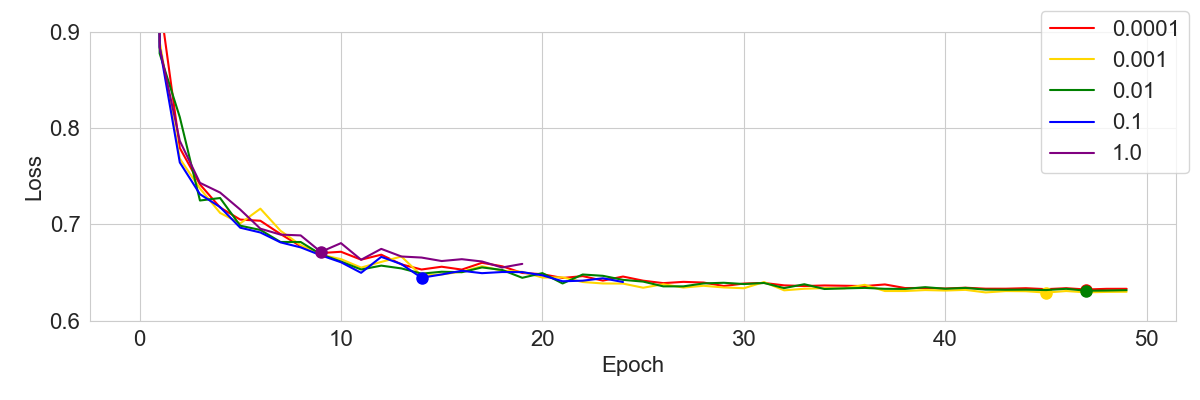
\includegraphics[height=55mm]{./figure/sec4/loss_curve/0/mel_loss.png}
        \caption{メルスペクトログラムのMAE Loss(式~\eqref{sec4:eq:loss}の$L_{mel}$)}
        \label{sec4:fig:method_1_val_mel_loss}
    \end{subfigure}
    \begin{subfigure}{\linewidth}
        \centering
        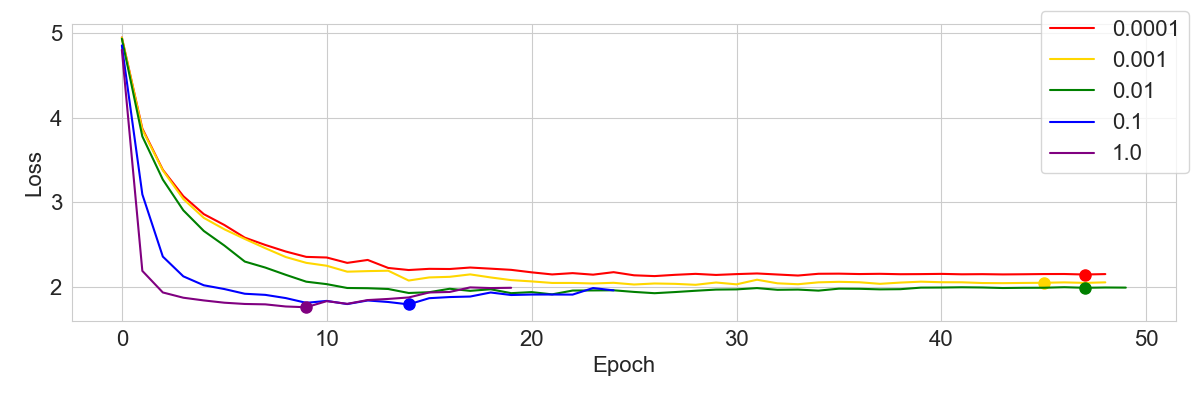
\includegraphics[height=55mm]{./figure/sec4/loss_curve/0/ssl_feature_cluster_loss.png}
        \caption{HuBERT離散特徴量のCross Entropy Loss(式~\eqref{sec4:eq:loss}の$L_{ssl^{d}}$)}
        \label{sec4:fig:method_1_val_ssl_feature_cluster_loss}
    \end{subfigure}
    \begin{subfigure}{\linewidth}
        \centering
        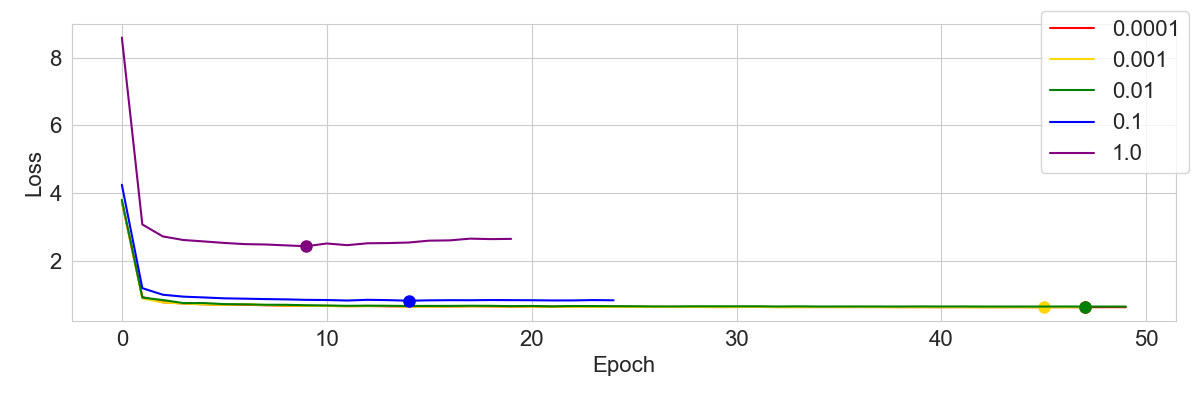
\includegraphics[height=55mm]{./figure/sec4/loss_curve/0/total_loss.png}
        \caption{損失の合計値(式~\eqref{sec4:eq:loss}の$L$)}
        \label{sec4:fig:method_1_val_total_loss}
    \end{subfigure}
    \caption{手法1における検証データに対する損失曲線}
    \label{sec4:fig:method_1_val_losses}
\end{figure}

\begin{figure}[bt]
    \centering
    \begin{subfigure}{\linewidth}
        \centering
        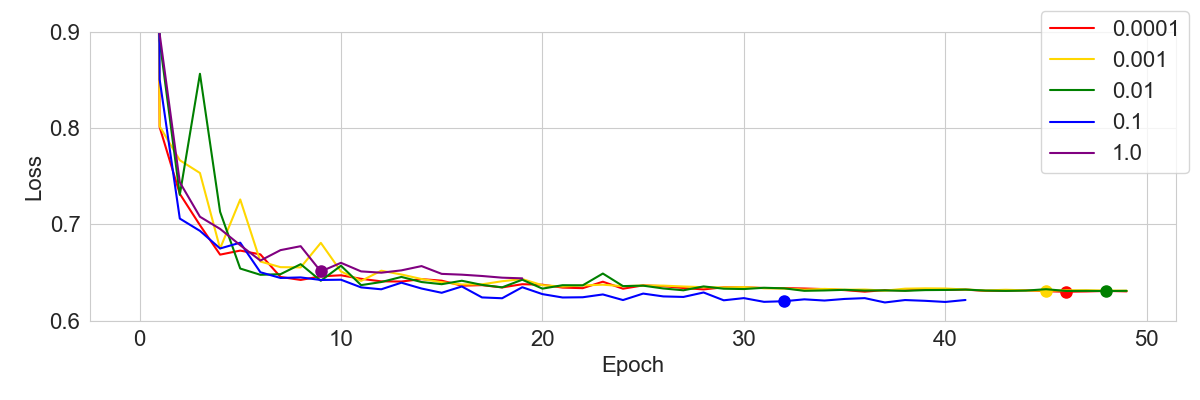
\includegraphics[height=55mm]{./figure/sec4/loss_curve/2/mel_loss.png}
        \caption{メルスペクトログラムのMAE Loss(式~\eqref{sec4:eq:loss}の$L_{mel}$)}
        \label{sec4:fig:method_2_val_mel_loss}
    \end{subfigure}
    \begin{subfigure}{\linewidth}
        \centering
        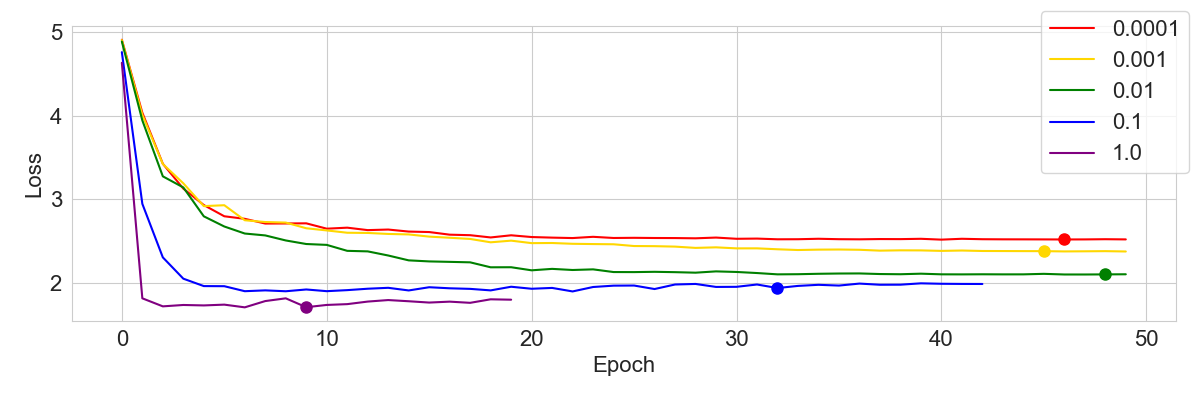
\includegraphics[height=55mm]{./figure/sec4/loss_curve/2/ssl_feature_cluster_loss.png}
        \caption{HuBERT離散特徴量のCross Entropy Loss(式~\eqref{sec4:eq:loss}の$L_{ssl^{d}}$)}
        \label{sec4:fig:method_2_val_ssl_feature_cluster_loss}
    \end{subfigure}
    \begin{subfigure}{\linewidth}
        \centering
        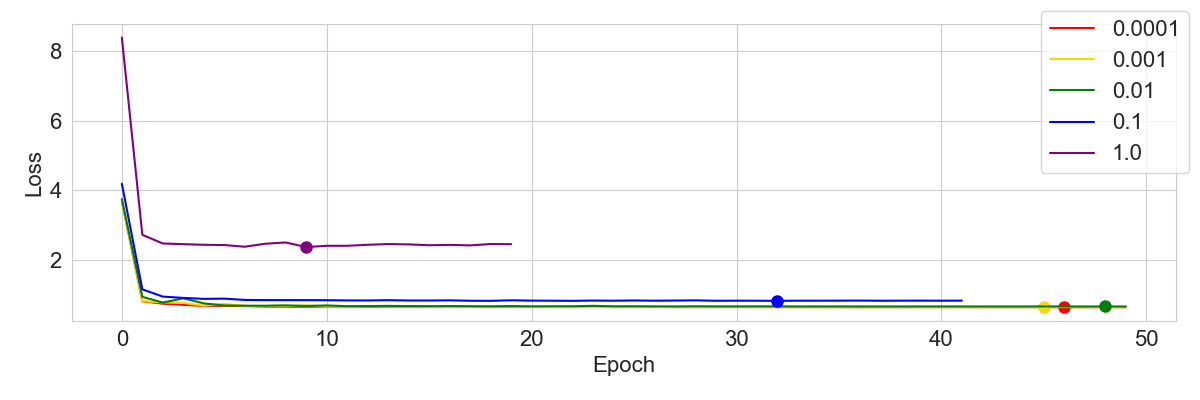
\includegraphics[height=55mm]{./figure/sec4/loss_curve/2/total_loss.png}
        \caption{損失の合計値(式~\eqref{sec4:eq:loss}の$L$)}
        \label{sec4:fig:method_2_val_total_loss}
    \end{subfigure}
    \caption{手法2における検証データに対する損失曲線}
    \label{sec4:fig:method_2_val_losses}
\end{figure}

\begin{figure}[bt]
    \centering
    \begin{subfigure}{\linewidth}
        \centering
        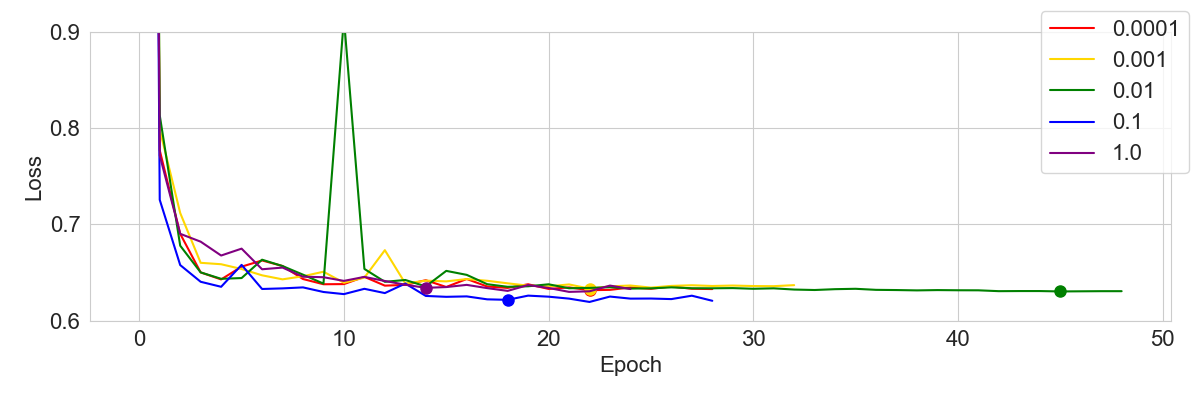
\includegraphics[height=55mm]{./figure/sec4/loss_curve/3/mel_loss.png}
        \caption{メルスペクトログラムのMAE Loss(式~\eqref{sec4:eq:loss}の$L_{mel}$)}
        \label{sec4:fig:method_3_val_mel_loss}
    \end{subfigure}
    \begin{subfigure}{\linewidth}
        \centering
        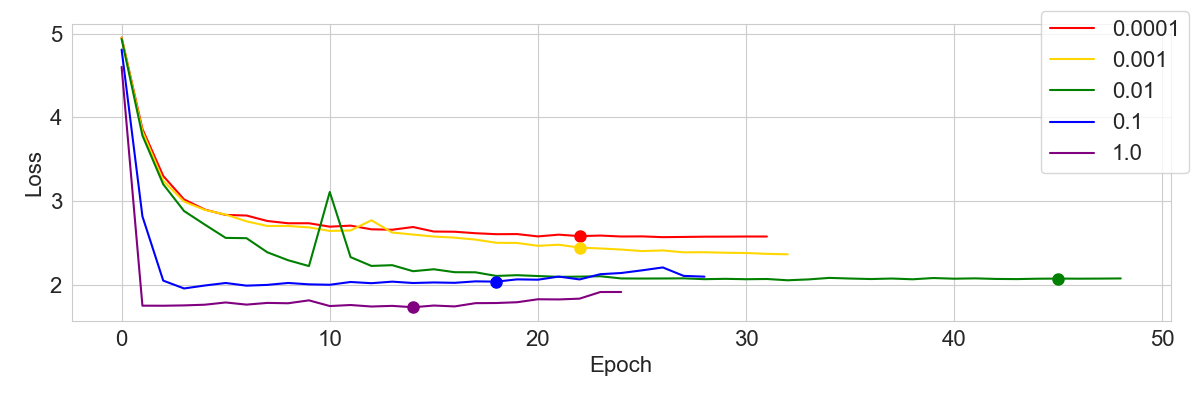
\includegraphics[height=55mm]{./figure/sec4/loss_curve/3/ssl_feature_cluster_loss.png}
        \caption{HuBERT離散特徴量のCross Entropy Loss(式~\eqref{sec4:eq:loss}の$L_{ssl^{d}}$)}
        \label{sec4:fig:method_3_val_ssl_feature_cluster_loss}
    \end{subfigure}
    \begin{subfigure}{\linewidth}
        \centering
        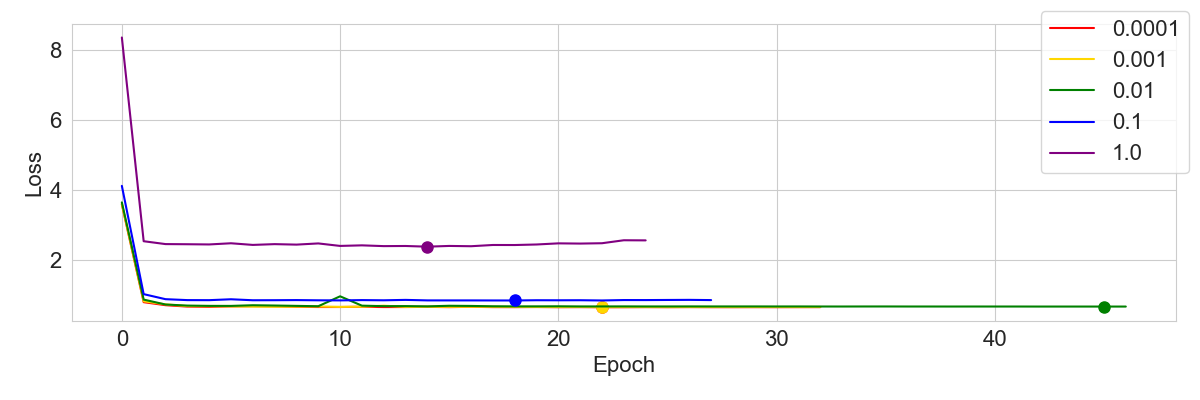
\includegraphics[height=55mm]{./figure/sec4/loss_curve/3/total_loss.png}
        \caption{損失の合計値(式~\eqref{sec4:eq:loss}の$L$)}
        \label{sec4:fig:method_3_val_total_loss}
    \end{subfigure}
    \caption{手法3における検証データに対する損失曲線}
    \label{sec4:fig:method_3_val_losses}
\end{figure}

\begin{figure}[bt]
    \centering
    \begin{subfigure}{\linewidth}
        \centering
        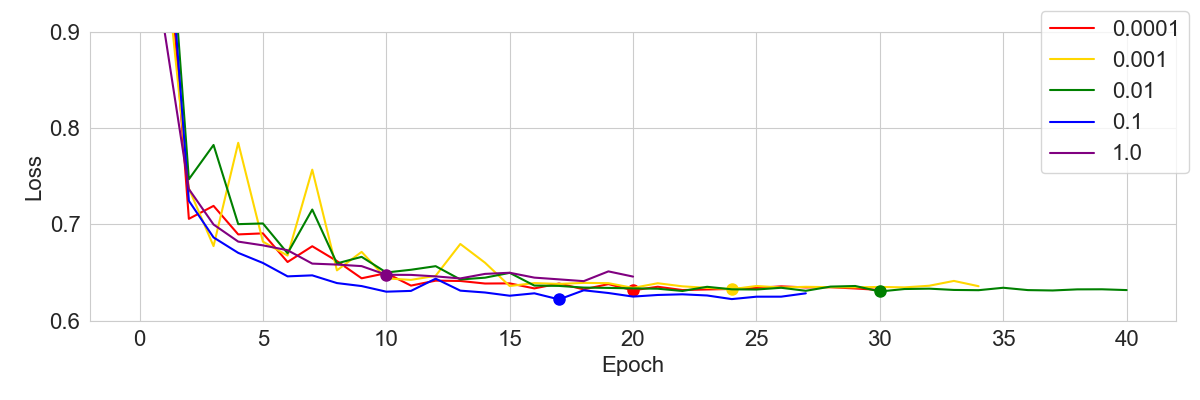
\includegraphics[height=55mm]{./figure/sec4/loss_curve/4/mel_loss.png}
        \caption{メルスペクトログラムのMAE Loss(式~\eqref{sec4:eq:loss}の$L_{mel}$)}
        \label{sec4:fig:method_4_val_mel_loss}
    \end{subfigure}
    \begin{subfigure}{\linewidth}
        \centering
        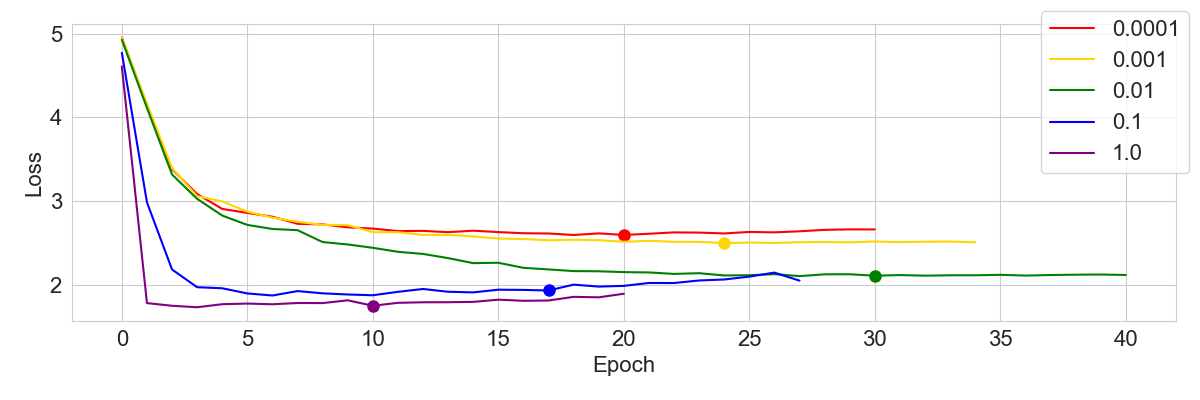
\includegraphics[height=55mm]{./figure/sec4/loss_curve/4/ssl_feature_cluster_loss.png}
        \caption{HuBERT離散特徴量のCross Entropy Loss(式~\eqref{sec4:eq:loss}の$L_{ssl^{d}}$)}
        \label{sec4:fig:method_4_val_ssl_feature_cluster_loss}
    \end{subfigure}
    \begin{subfigure}{\linewidth}
        \centering
        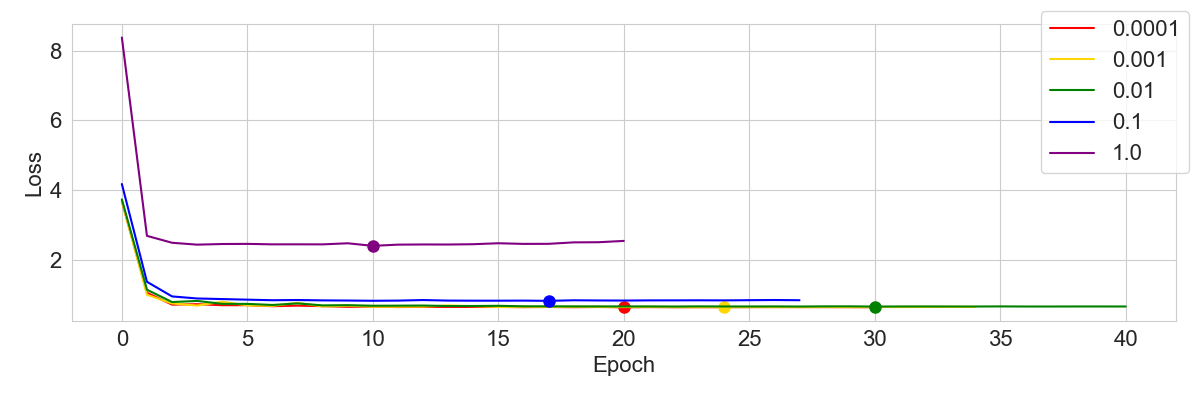
\includegraphics[height=55mm]{./figure/sec4/loss_curve/4/total_loss.png}
        \caption{損失の合計値(式~\eqref{sec4:eq:loss}の$L$)}
        \label{sec4:fig:method_4_val_total_loss}
    \end{subfigure}
    \caption{手法4における検証データに対する損失曲線}
    \label{sec4:fig:method_4_val_losses}
\end{figure}

\begin{figure}[bt]
    \centering
    \begin{subfigure}{\linewidth}
        \centering
        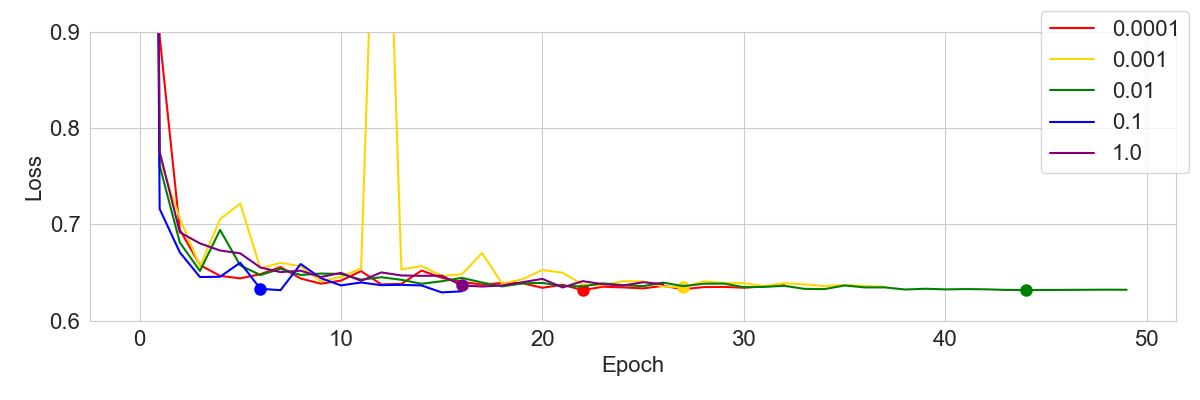
\includegraphics[height=55mm]{./figure/sec4/loss_curve/5/mel_loss.png}
        \caption{メルスペクトログラムのMAE Loss(式~\eqref{sec4:eq:loss}の$L_{mel}$)}
        \label{sec4:fig:method_5_val_mel_loss}
    \end{subfigure}
    \begin{subfigure}{\linewidth}
        \centering
        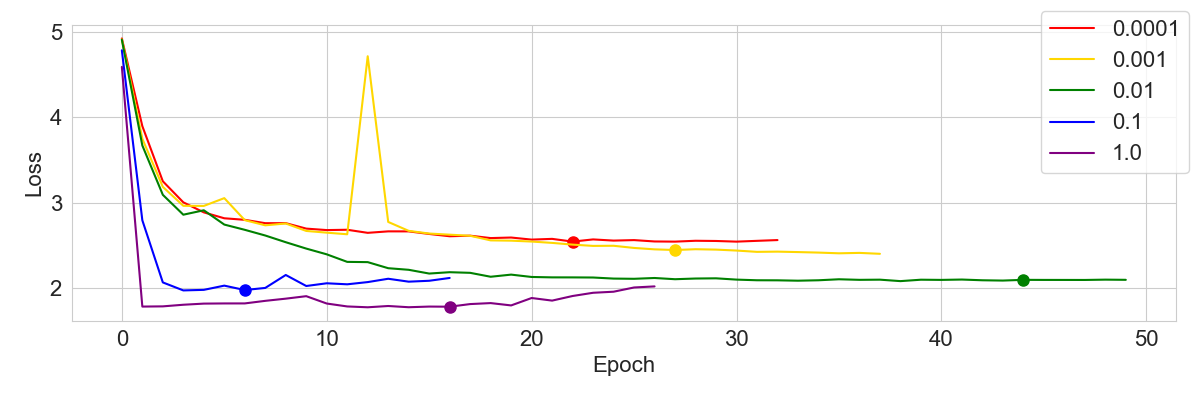
\includegraphics[height=55mm]{./figure/sec4/loss_curve/5/ssl_feature_cluster_loss.png}
        \caption{HuBERT離散特徴量のCross Entropy Loss(式~\eqref{sec4:eq:loss}の$L_{ssl^{d}}$)}
        \label{sec4:fig:method_5_val_ssl_feature_cluster_loss}
    \end{subfigure}
    \begin{subfigure}{\linewidth}
        \centering
        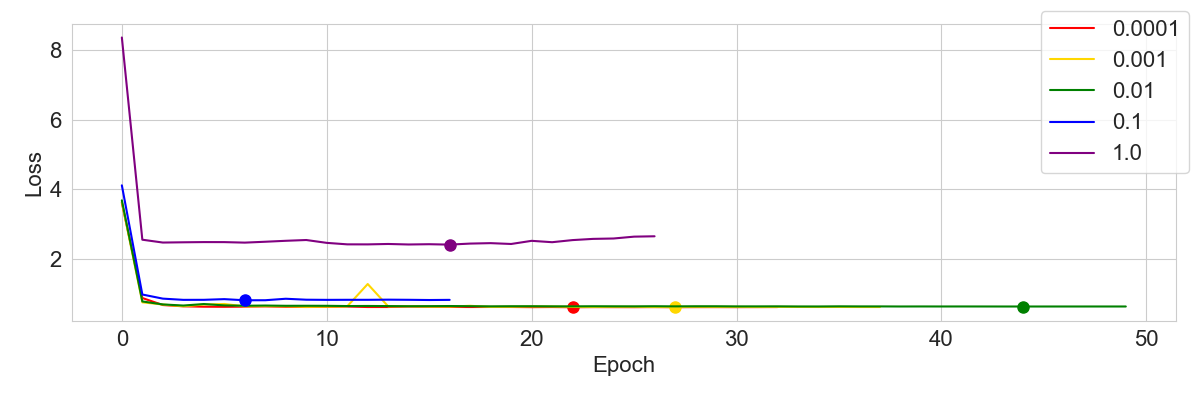
\includegraphics[height=55mm]{./figure/sec4/loss_curve/5/total_loss.png}
        \caption{損失の合計値(式~\eqref{sec4:eq:loss}の$L$)}
        \label{sec4:fig:method_5_val_total_loss}
    \end{subfigure}
    \caption{手法5における検証データに対する損失曲線}
    \label{sec4:fig:method_5_val_losses}
\end{figure}

\begin{table*}[bt]
    \centering
    \caption{最適なチューニングをした場合における手法ごとの比較}
    \label{sec4:tab:obj_method_comp}
    \begin{center}
        \renewcommand{\arraystretch}{1.0} % 行の高さ調整
        \setlength{\tabcolsep}{8pt}      % 列の幅調整
        \scalebox{0.88}{
            \begin{tabular}{|l|l|rr|}
                \hline
                \multicolumn{1}{|c|}{手法} & \multicolumn{1}{c|}{詳細}  & \multicolumn{1}{c}{WER [\%]} & \multicolumn{1}{c|}{話者類似度} \\
                \hline
                1                        & ベースライン                   & 55.4                         & 0.845                      \\
                2                        & 事前学習なしTransformer        & 46.1                         & 0.845                      \\
                3                        & 事前学習なしTransformer・アンサンブル & \underline{45.7}             & \underline{0.848}          \\
                4                        & 事前学習ありTransformer        & 47.0                         & 0.833                      \\
                5                        & 事前学習ありTransformer・アンサンブル & 46.8                         & 0.822                      \\
                \hline
                6                        & 分析合成                     & 4.7                          & 0.926                      \\
                7                        & 原音声                      & 4.5                          & 1.000                      \\
                \hline
            \end{tabular}
        }
    \end{center}
\end{table*}

\subsubsection{主観評価}

\subsection{まとめ}
\clearpage

% \section{音声SSLモデルを活用した動画音声合成の検討}
% \label{音声SSLモデルを活用した動画音声合成の検討}
% 本章では、音声SSLモデルであるHuBERTを利用した動画音声合成モデルを提案する。実験では比較手法として先行研究\cite{choi2023intelligible}のアプローチを含みつつ、モデルの予測対象についても複数検討した。

% \subsection{音声合成法}
% 提案手法の構築手順は二段階に分かれる。ネットワークの概要を図~\ref{sec4:fig:network}に示す。まず、動画を入力として、メルスペクトログラムとHuBERT中間特徴量を推定するネットワークを学習する(図~\ref{sec4:fig:network}-A)。HuBERT中間特徴量は、HuBERTにおける畳み込み層出力のことを指す。ここでは、AVHuBERTを動画からの特徴抽出に利用した。AVHuBERTにはパラメータ数が1億程度のBaseモデルと、3億程度のLargeモデルが存在するが、本研究では計算機のメモリの都合上、Baseモデルのみを検討した。AVHuBERTへの音声特徴量は、先行研究と同様に0で埋めた特徴量を入力した。これによって動画のみを入力した下流タスクへのFineTuningが可能となる。この出力に対して、手法~\cite{wan2018generalized}によって音声波形から得られる話者Embeddingをチャンネル方向に結合する。その後、畳み込み層からなるデコーダを通すことによって、話者Embeddingを新たに結合した特徴量に対する変換を施した。デコーダは残差結合を利用したブロック単位で構成され、各ブロックに2層の畳み込み層を設けた。畳み込み層のカーネルサイズは3とし、2ブロック積み重ねた。最後に、全結合層に通すことによって所望の出力を得る。一度チャンネルサイズ \texttimes 出力特徴量のフレーム数まで次元を拡張し、その後reshapeすることによって所望の次元、フレーム数となった最終出力を得た。

% 次に、一段階目に学習されたネットワークの重みを固定した状態でHuBERT中間特徴量を推定し、それを入力としてHuBERTのTransformer層の学習を行う(図~\ref{sec4:fig:network}-B)。ここでは、原音声から計算されたHuBERT出力特徴量(音声SSL特徴量)を推定対象とする。HuBERTの自己教師あり学習においてマスクが適用されるのは畳み込み層出力であるため、その後のTransformer層を本研究のタスクにFine Tuningすることにより、推定残差の軽減を狙った。予測対象として以下三種類を検討した。
% \begin{enumerate}
%     \item 音声SSL特徴量の連続値自体をそのまま予測対象とする場合(音声SSL連続特徴量)
%     \item 音声SSL特徴量をk-means法によるクラスタリングで離散化し、そのクラスタを予測対象とする場合(音声SSL離散特徴量)
%     \item 上記二つのマルチタスク学習の場合
% \end{enumerate}

% 以上のモデルを組み合わせることで、動画から音響特徴量の推定が可能になる。具体的には、一段階目に得られるモデルに動画を入力することでメルスペクトログラムとHuBERT中間特徴量を推定し、そのうちHuBERT中間特徴量をFineTuningされたHuBERTのTransformer層に入力することで、音声SSL特徴量が得られる。その後、先行研究~\cite{choi2023intelligible}に基づくMulti-input Vocoderを用い、メルスペクトログラムと音声SSL特徴量を入力として音声波形に変換することで、最終的な合成音声を得たMulti-input VocoderはHifi-gan~\cite{kong2020hifi}をベースとしたモデルである。本研究では動画から予測される音響特徴量が複数パターン存在するため、そのパターンごとに別個でボコーダを学習した。

% \begin{figure}[bt]
%     \centering
%     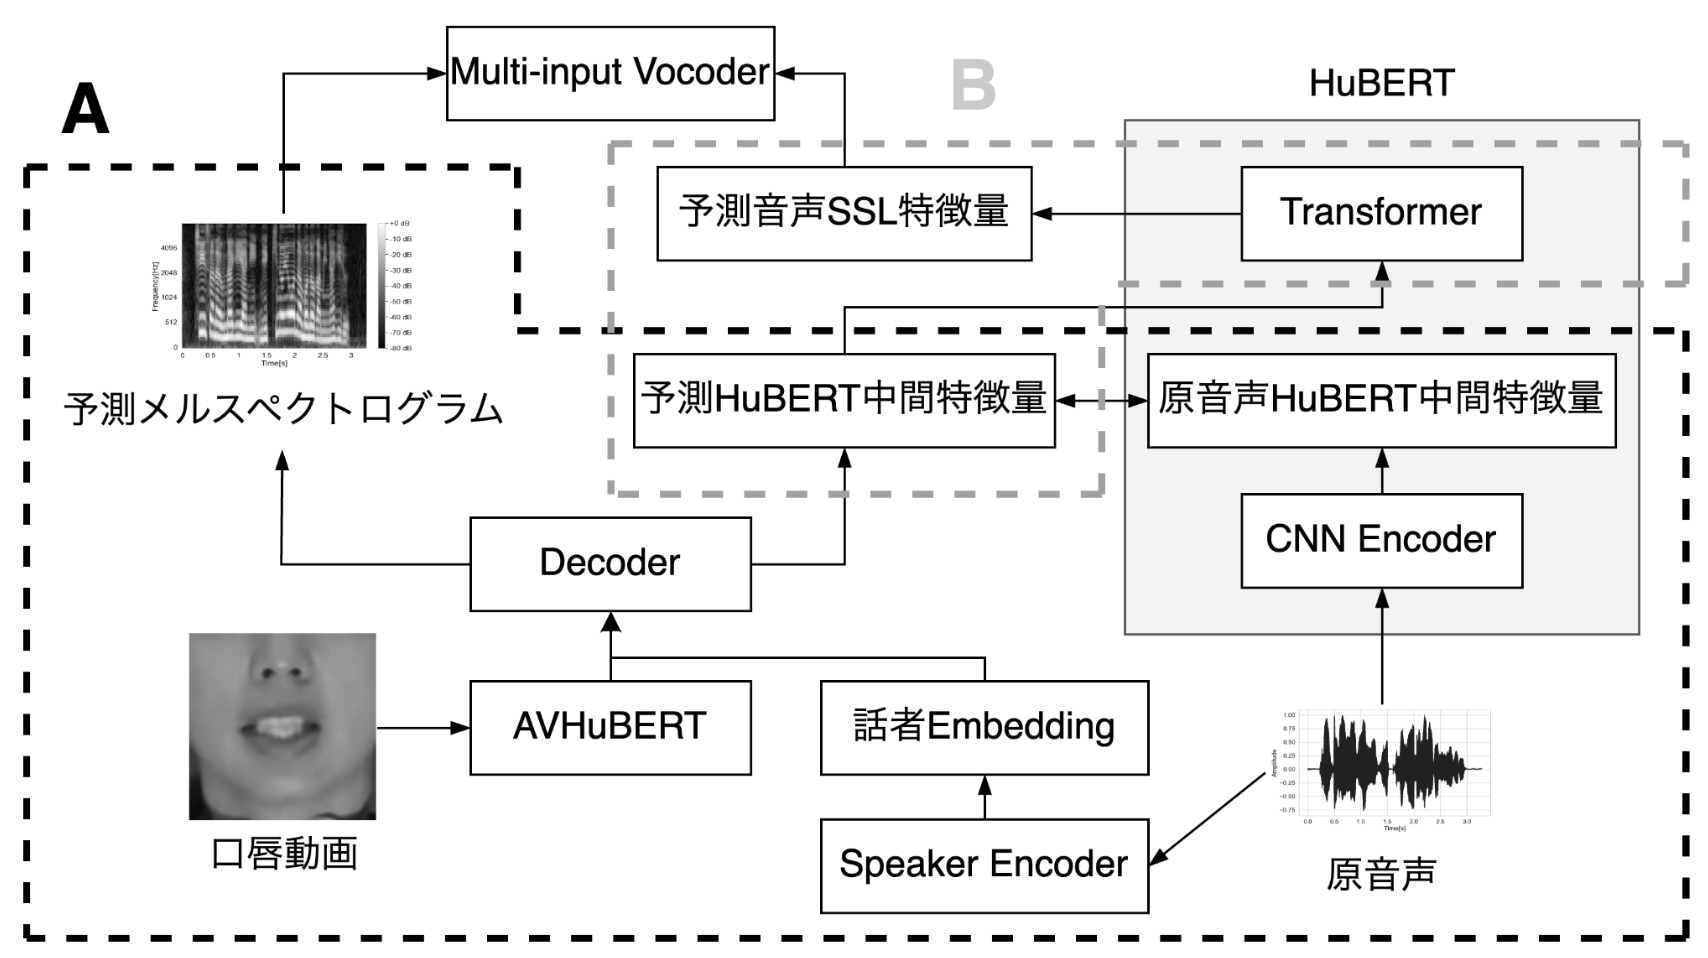
\includegraphics[height=90mm]{./figure/sec4/network.png}
%     \caption{ネットワークの概略図}
%     \label{sec4:fig:network}
% \end{figure}

% \subsection{実験方法}
% \subsubsection{利用したデータセット}
% 動画音声データセットには、男女二人ずつから収録した合計4人分のデータセット~\cite{taguchi,esaki}を用いた。これはATR音素バランス文~\cite{atr}から構成され、全話者共通でAからHセットを学習データ、Iセットを検証データ、Jセットをテストデータとして利用した。各分割ごとの文章数を表~\ref{sec4:tab:dataset_info}に示す。

% Multi-input Vocoderの学習に利用する音声データセットには、Hi-Fi-Captain(日本語話者二名分)~\cite{okamoto2023hi}とJVS(parallel100とnonpara30)~\cite{takamichi2019jvs}を利用した。ボコーダの学習時にはサンプル全体から1秒分をランダムにサンプリングして用いるのだが、元データには話し声のない無音区間が一定存在しており、これはボコーダの学習に望ましくない。これに対して、無音区間のトリミング(-40 dBFS未満かつ500 ms継続する区間を100 msまでカット)を適用した。Hi-Fi-Captainはtrain-parallelおよびtrain-non-parallelを学習データ、valを検証データ、evalをテストデータとして分割した。各分割ごとの文章数を表~\ref{sec4:tab:dataset_info}に示す。JVSには話者に対して1から100まで番号が割り振られており、本実験では1から80番の話者を学習データ、81番から90番の話者を検証データ、91番から100番までの話者をテストデータとした。各分割ごとの文章数を表~\ref{sec4:tab:dataset_info}に示す。

% \begin{table*}[bt]
%     \centering
%     \caption{利用したデータセットの文章数}
%     \label{sec4:tab:dataset_info}
%     \begin{center}
%         \renewcommand{\arraystretch}{0.9} % 行の高さ調整
%         \setlength{\tabcolsep}{8pt}      % 列の幅調整
%         \scalebox{1.0}{
%             \begin{tabular}{|l|r|r|r|}
%                 \hline
%                               & \multicolumn{1}{c|}{学習} & \multicolumn{1}{c|}{検証} & \multicolumn{1}{c|}{テスト} \\
%                 \hline
%                 動画音声データセット    & 1600                    & 200                     & 212                      \\
%                 Hi-Fi-Captain &                         &                         &                          \\
%                 JVS           &                         &                         &                          \\
%                 \hline
%             \end{tabular}
%         }
%     \end{center}
% \end{table*}

% \subsubsection{データの前処理}
% 動画データは60 FPSで収録されたものをffmpegにより25 FPSに変換して用いた。その後、手法~\cite{bulat2017far}により動画に対してランドマーク検出を適用した。このランドマークを利用することで口元のみを切り取り、画像サイズを(96, 96)にリサイズした上で、グレースケールに変換した。加えて、画像に対する正規化および標準化を適用した。学習時は、ランダムクロップ、左右反転、Time Masking(一時停止)をデータ拡張として適用した。ランダムクロップは、(96, 96)で与えられる画像から(88, 88)をランダムに切り取る処理である。検証およびテスト時は、必ず画像中央を切り取るよう実装した。左右反転はランダムクロップ後に適用しており、50\%の確率で左右が反転されるよう実装した。Time Maskingは、連続する画像の時間平均値を利用することによって、一時停止させるような効果を与えるデータ拡張手法である。動画1秒あたり0から0.5秒の間でランダムに停止区間を定め、その区間における動画の時間方向平均値を計算し、区間内のすべてのフレームをこの平均値で置換した。

% 音声データは48 kHzで収録されたものを16 kHzにダウンサンプリングして用いた。それから、窓長25 msのハニング窓を用いて、シフト幅10 msでSTFTを適用することでフレームレート100 Hzのスペクトログラムに変換した。さらに、振幅スペクトログラムに対して80次のメルフィルタバンクを適用し、80次のメルスペクトログラムを得た上で対数スケールに変換した。話者Embeddingの取得には事前学習済みモデル~\cite{wan2018generalized}を利用し、学習データから100個ランダムサンプリングして計算した平均値を利用した。

% HuBERTは、HuggingFaceに公開されているReazonSpeechというデータセットによって学習されたモデル~\cite{rinna-japanese-hubert-base,sawada2024release}を利用した。ReazonSpeechは約19000時間の日本語音声からなるデータセットであり、日本語音声のコンテキストを大量のデータから学習したモデルになっていることが予想される。本研究のアプローチでは、日本語音声に関する事前知識を豊富に有するモデルが適していると考え、このモデルを選択した。検討した予測対象の一つである音声SSL離散特徴量は、k-means法によるクラスタリング(クラスタ数200)によって得た。クラスタ数は、今回比較する先行研究~\cite{choi2023intelligible}に基づいている。このモデルの学習にはHi-Fi-Captainを利用しており、男性女性それぞれ学習データ全体から50\%をランダムサンプリングして用いた。

% \subsubsection{学習方法}
% 第一段階であるAVHuBERTをベースとしたモデルの学習について、損失関数はメルスペクトログラムについてのMAE Lossと、HuBERT中間特徴量のMAE Lossの和とした。最適化手法にはAdamW~\cite{loshchilov2017decoupled}を利用し、$\beta_{1} = 0.9$、$\beta_{2} = 0.98$、$weight\_decay = 0.01$とした。学習率は\num{1.0e-3}から開始し、Warmup Schedulerによってその値を変化させた。バッチサイズはメモリの都合上4としたが、学習の安定のためGradient Accumulationによって各イテレーションにおける勾配を累積させ、8イテレーションに一回重みを更新するようにした。そのため、実質的にはバッチサイズ32となる。モデルに入力する動画の秒数は10秒を上限とし、それを超える場合はランダムにトリミング、それに満たない場合はゼロパディングした。勾配のノルムは3.0を上限としてクリッピングすることで、過度に大きくなることを防止した。最大エポック数は50とし、10エポック連続して検証データに対する損失が小さくならない場合には、学習を中断するようにした。また、学習終了時には検証データに対する損失が最も小さかったエポックにおけるチェックポイントを保存し、これをテストデータに対する評価に用いた。

% 第二段階であるHuBERTをベースとしたモデルの学習について、音声SSL連続特徴量に対する損失関数にはMAE Loss、音声SSL離散特徴量に対する損失関数にはCross Entropy Lossを使用した。マルチタスク学習を行う場合には、Cross Entropy Lossに対して重み係数をかけることでチューニングを行った。従って、マルチタスク学習時の損失関数は以下のように表される。
% \begin{equation}
%     L = L_{c} + \lambda * L_{d}
%     \label{sec4:eq:loss_}
% \end{equation}
% $L_{c}$はMAE Loss、$L_{d}$はCross Entropy Lossであり、$\lambda$がCross Entropy Lossにかかる重み係数を表す。本実験では$\lambda = \num{1.0e-4}$から1.0まで、10倍刻みで5段階検討した。
% 最適化手法にはAdamWを利用し、$\beta_{1} = 0.9$、$\beta_{2} = 0.98$、$weight\_decay = 0.01$とした。学習率は\num{5.0e-4}から開始し、Warmup Schedulerによってその値を変化させた。その他学習に関わるパラメータは、第一段階における値と同じである。

% Multi-input Vocoderの学習について、これは入力される音響特徴量のバリエーションに対してそれぞれ別個にモデルを構築した。全てをまとめると以下の通りである。
% \begin{enumerate}
%     \item メルスペクトログラム
%     \item メルスペクトログラム $+$ 音声SSL連続特徴量
%     \item メルスペクトログラム $+$ 音声SSL離散特徴量
%     \item メルスペクトログラム $+$ 音声SSL連続特徴量 $+$ 音声SSL離散特徴量
% \end{enumerate}
% 学習は動画音声データセットではなく、外部データであるHi-Fi-CaptainとJVSを用いた。はじめにHi-Fi-Captainのみを用いて学習させ、その後学習済みモデルをJVSによって再学習した。Hi-Fi-Captainは男女一人ずつの文章数が豊富なデータセットであるため、高品質なモデルを構築可能であった。しかし、学習できる話者数が少ない分、学習外話者に対する合成音声の品質が低かった。そのため、一人当たりの文章数は100文章程度と少ないながらも、100人分の話者からなるJVSを利用して再学習することによって、学習外話者に対する合成音声の品質を向上させた。最適化手法にはAdamWを利用し、$\beta_{1} = 0.8$、$\beta_{2} = 0.99$、$weight_decay = 0.01$とした。学習率は\num{2.0e-4}から開始し、指数関数的にその値を変化させた。バッチサイズは16とし、ここではGradient Accumulationは利用しなかった。モデルへの入力は1秒を上限とし、それを超える場合はランダムにトリミング、それに満たない場合はゼロパディングした。勾配のノルムは3.0を上限としてクリッピングすることで、過度に大きくなることを防止した。最大エポック数は30とし、ここではEarly Stoppingは適用しなかった。また、学習終了時には検証データに対する損失(メルスペクトログラムに対するL1 Loss)が最も小さかったエポックにおけるチェックポイントを保存し、これをテストデータに対する評価に用いた。

% GPUはNVIDIA RTX A4000を利用し、計算の高速化のためAutomatic Mixed Precisionを適用した。

% \subsubsection{比較手法}
% \label{比較手法}
% 比較手法は、メルスペクトログラムのみを予測対象とするベースライン、HuBERTなしのマルチタスク学習手法~\cite{choi2023intelligible}、HuBERTありのマルチタスク学習手法(提案手法)の三種類である。ただし、マルチタスク学習手法の予測対象には、以下の三種類が存在する。
% \begin{enumerate}
%     \item 音声SSL連続特徴量
%     \item 音声SSL離散特徴量
%     \item 音声SSL連続特徴量 $+$ 音声SSL離散特徴量
% \end{enumerate}
% HuBERTなしのマルチタスク学習手法、HuBERTありのマルチタスク学習手法には上記3パターンを設けたため、比較したのは計7手法となる。

% \subsubsection{客観評価}
% 合成音声の客観評価には、PESQ~\cite{rix2001perceptual}、STOI~\cite{taal2010short}、ESTOI~\cite{taal2011algorithm}、WERの4種類の客観評価指標を使用した。PESQは音声の自然性を表す指標であり、1から5の値を取る。値が高いほど良い。STOI、ESTOIはどちらも音声の明瞭性を表す指標であり、0から1の値を取る。PESQと同様に、値が高いほど良い。ここまでの三つの指標は、TorchMetricsというライブラリを用いて算出した。WERは、Whisper~\cite{radford2023robust}による音声認識の結果から算出した単語誤り率である。合成音声がより正確に認識されるほど聞き取りやすいと考えられるため、この指標は値が低いほど良い。この計算方法については、まず、Whisperによって出力されるテキストに対して、句読点を削除した上でMeCab (日本語形態素解析エンジン)を用いて分かち書きを行い、単語に分解する。その後、jiwerというライブラリを用いてWERを計算した。

% \subsubsection{主観評価}

% \begin{figure}[bt]
%     \centering
%     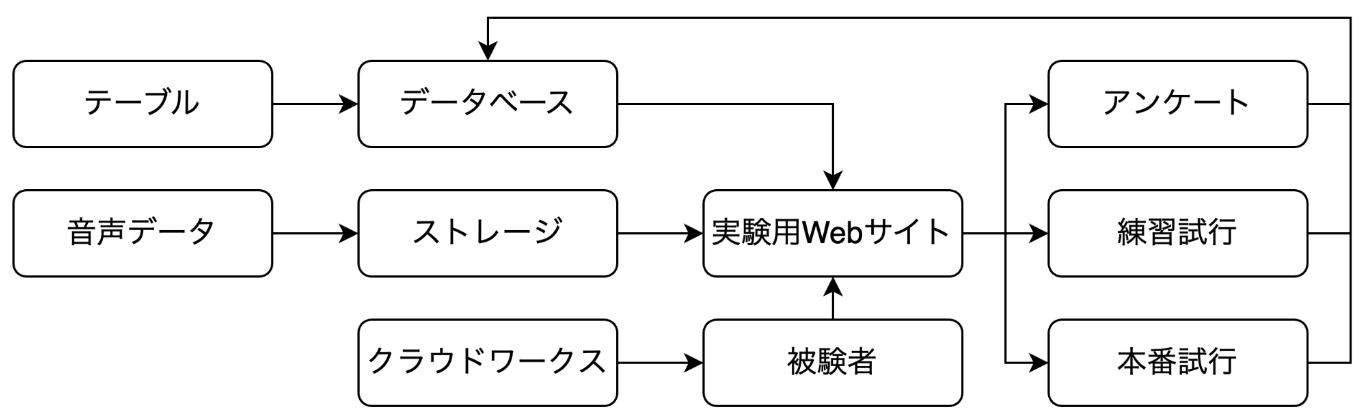
\includegraphics[height=45mm]{./figure/sec4/sbj_flow.png}
%     \caption{主観評価実験全体の流れ}
%     \label{sec4:fig:sbj_flow}
% \end{figure}

% 主観評価実験では、音声の明瞭性と自然性を実際に人に聞いていただくことで評価した。実験全体の流れを図~\ref{sec4:fig:sbj_flow}に示す。今回はクラウドワークスというクラウドソーシングサービスおよび、自作の実験用 Web サイトを利用して、オンラインで実験を実施した。実験全体の大まかな流れは以下の通りである。
% \begin{enumerate}
%     \item 音声ファイルをクラウドストレージにアップロードするとともに、実験データを管理するためのテーブルをリモートサーバーのデータベースに作成する。
%     \item クラウドワークスにて実験を公開し、被験者を募集する。
%     \item 被験者と契約後、実験用Webサイトから実験を実施していただく。結果はデータベースに格納する。
%     \item 実験終了後、データベースから評価データを取得して統計処理を実施する。
% \end{enumerate}
% 被験者の方に行っていただいた項目は以下の三つである。
% \begin{enumerate}
%     \item アンケート
%     \item 練習試行
%     \item 本番試行
% \end{enumerate}
% 一つ目のアンケートでは、被験者についての基本的な統計を取ることを目的として、性別・年齢・利用した音響機器について回答していただいた。二つ目の練習試行では、実験本番の前に実験内容を把握していただくことを目的として、練習用の実験を行っていただいた。三つ目の本番試行では、最終的に統計処理に利用する評価データを得るための、本番の実験を実施した。

% 評価項目の一つである明瞭性について、教示は以下のように行った。
% \begin{quote}
%     一つ目の評価項目である明瞭性は、\textbf{発話内容自体がどれくらい聞き取りやすかったか}を指します。

%     この評価は自然性とは異なり、発話内容の理解のしやすさに焦点を当てています。

%     各音声ごとに、下記の五段階で評価してください。
%     \begin{enumerate}
%         \item 非常に悪い
%         \item 悪い
%         \item 普通
%         \item 良い
%         \item 非常に良い
%     \end{enumerate}
% \end{quote}
% もう一つの評価項目である自然性について、教示は以下のように行った。
% \begin{quote}
%     二つ目の評価項目である自然性は、\textbf{発話内容によらず、その音声がどれくらい人間らしく自然なものに聞こえたか}を指します。

%     例えば、音質自体やイントネーションの自然さなどが評価の観点として挙げられます。

%     イントネーションなど発話内容に関連する要素も含まれますが、ここではどれくらい自然な音声であるかを評価してください。

%     発話内容の聞き取りやすさではなく、音声全体の自然さが評価の対象です。この点が明瞭性の評価と異なる部分です。

%     各音声ごとに、下記の五段階で評価してください。
%     \begin{enumerate}
%         \item 非常に悪い
%         \item 悪い
%         \item 普通
%         \item 良い
%         \item 非常に良い
%     \end{enumerate}
% \end{quote}
% 自然性は明瞭性よりも漠然としており、先行研究でも教示の仕方によって評価の傾向が変化することが報告されている\cite{dall2014rating}。そのため、自然性の教示では音質やイントネーションなど、具体的に評価していただきたい観点を示した。

% 評価対象は、~\ref{比較手法}節に示した7手法に分析合成、原音声を加えた9種類の音声である。分析合成は、原音声から計算した特徴量を入力として、Multi-input Vocoderで逆変換した合成音声である。これは、今回構築したニューラルボコーダ自体の性能を表す値であり、今回の実験における合成音声の品質上限を表すような手法である。評価文章は客観評価と同様に、ATR音素バランス文のJセット53文章を利用し、話者は学習に用いた4人分全てを用いた。すなわち、各手法ごとに212サンプル($= 53 \text{文章} \times 4 \text{話者}$)を利用した。被験者ごとの評価サンプルの割り当て方法を以下に述べ、図\ref{sec4:fig:sbj_selection}にその概要も示す。
% \begin{enumerate}
%     \item 評価に用いる53文章を9つ(評価手法の総数)のグループにランダムに分割する。各グループごとに一文章を練習試行用、それ以外の文章を本番試行用としてランダムに割り振る。
%     \item 各文章グループに一つ手法を割り当て、文章一つ一つに対して話者を一人ランダムに選択する。これにより、ある被験者一名に対してユニークな53文章からなる評価データが得られる。
% \end{enumerate}
% 上記に加えて、被験者ごとに文章グループに割り当てる手法を一つずつずらすよう実装した。この過程を表\ref{sec4:tab:sbj_selection_relation}に示す。被験者ごとに文章グループに対して割り当てる手法を1ずつずらしていくことで、文章と手法の組み合わせを効率よく網羅できるようにした\cite{king2008blizzard}。加えて、サンプル選択の過程では、すべての組み合わせについて以前に評価された回数をカウントしておくことで、サンプルの選択にランダム性を持たせつつ、すべてのサンプルが等しい回数評価されるようにした。例えば、一回選択されたサンプルと未選択のサンプルが存在する場合、一回選択されたサンプルは選択の候補から除外する。これにより、未選択のサンプルのみを対象としたランダムサンプリングを行うことで、最終的な評価回数が等しくなるよう実装した。この選択方法により、36回の実験によって$\text{(手法)} \times \text{(文章)} \times \text{(話者)}$のすべての組み合わせが一回ずつ評価されることになる。

% \begin{figure}[bt]
%     \centering
%     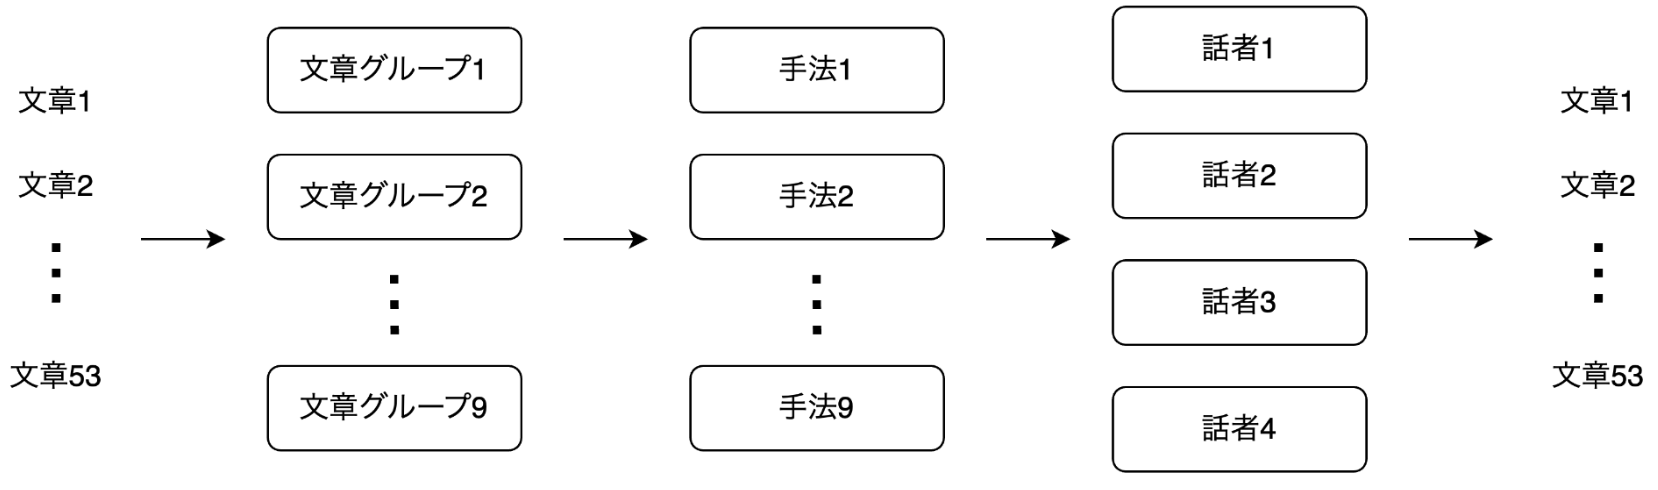
\includegraphics[height=45mm]{./figure/sec4/sbj_selection.png}
%     \caption{主観評価実験における話者ごとのサンプル選択}
%     \label{sec4:fig:sbj_selection}
% \end{figure}

% \begin{table*}[bt]
%     \centering
%     \caption{主観評価実験のサンプル選択における文章グループと手法の対応関係}
%     \label{sec4:tab:sbj_selection_relation}
%     \begin{center}
%         \renewcommand{\arraystretch}{1.0} % 行の高さ調整
%         \setlength{\tabcolsep}{8pt}      % 列の幅調整
%         \scalebox{0.9}{
%             \begin{tabular}{|c|ccccccccc|}
%                 \hline
%                 \multirow{2}{*}{}         & \multicolumn{9}{c|}{文章グループインデックス}                                 \\
%                                           & 1                                 & 2 & 3 & 4 & 5 & 6 & 7 & 8 & 9 \\
%                 \hline
%                 \multirow{9}{*}{手法インデックス} & 1                                 & 2 & 3 & 4 & 5 & 6 & 7 & 8 & 9 \\
%                                           & 2                                 & 3 & 4 & 5 & 6 & 7 & 8 & 9 & 1 \\
%                                           & 3                                 & 4 & 5 & 6 & 7 & 8 & 9 & 1 & 2 \\
%                                           & 4                                 & 5 & 6 & 7 & 8 & 9 & 1 & 2 & 3 \\
%                                           & 5                                 & 6 & 7 & 8 & 9 & 1 & 2 & 3 & 4 \\
%                                           & 6                                 & 7 & 8 & 9 & 1 & 2 & 3 & 4 & 5 \\
%                                           & 7                                 & 8 & 9 & 1 & 2 & 3 & 4 & 5 & 6 \\
%                                           & 8                                 & 9 & 1 & 2 & 3 & 4 & 5 & 6 & 7 \\
%                                           & 9                                 & 1 & 2 & 3 & 4 & 5 & 6 & 7 & 8 \\
%                 \hline
%             \end{tabular}
%         }
%     \end{center}
% \end{table*}

% 被験者数および各手法の評価回数に関して、先行研究\cite{wester2015we}では統計処理に用いる被験者数や評価回数を変数として、実験条件に対してどれほどの被験者数とサンプル数が必要そうであるかを検討している。今回はこの結果を参考に、オンラインで実験を実施するのであれば総被験者数が100人以上、各手法に対する総評価回数が200回以上となることが望ましいと判断した。前述したサンプル選択アルゴリズムにより、36回の実験によって全てのサンプルが一回ずつ評価される。これを1セットとすると、セットあたり被験者数は36人、各手法に対する評価回数は176回となる。従って、今回は3セット行うことにより、総被験者数108人、各手法に対しての総評価回数が528回となるようにした。実験一回あたり15分程度で終わると見積もって、一人当たりの報酬は250円とした。

% また、オンラインでの評価は効率よく数多くの方に評価していただけるという点でメリットがあるが、オフラインでの評価と比較して実験環境を制御することが難しく、評価の品質に不安が残る。これに対して、本実験では先行研究\cite{kirkland2023stuck}を参考に、評価サンプル中にダミー音声を混入させることで対策を講じた。ダミー音声は本研究で得られた合成音声とは無関係に、Googleのテキスト音声合成システムによって生成したサンプルである。このサンプルでは、
% \begin{quote}
%     これはダミー音声です。明瞭性は「2: 悪い」を、自然性は「1: 非常に悪い」を選択してください。
% \end{quote}
% のような音声が提示される。この時、その音声自体の明瞭性や自然性に関係なく、必ずこの音声によって指定された評価値を選択するよう教示を与えた。また、本番試行においてダミー音声で指定された評価値を誤って選んだ場合は、すべての回答を無効にし、報酬も支払うことができない旨を被験者に伝えた。実際の教示は以下のようなものである。
% \begin{quote}
%     音声サンプル内には、ダミー音声が含まれています。ダミー音声では、以下のような音声が再生されます。

%     「これはダミー音声です。明瞭性は〇〇を、自然性は〇〇を選択してください。」

%     再生した音声がダミー音声であった場合、必ずこの音声で指定された評価値を選択してください。これは、実験において適当な回答を防止するためのものです。

%     例として、下記の音声では、「これはダミー音声です。明瞭性は「2: 悪い」を、自然性は「1: 非常に悪い」を選択してください。」と指定しています。

%     (再生可能な音声サンプル)

%     この場合、明瞭性は「2: 悪い」、自然性は「1:非常に悪い」を選択します。音声自体の明瞭性や自然性を評価するわけではないため、ご注意ください。

%     特に、\textbf{本番試行においてダミー音声で指定された評価値を誤って選んだ場合は、全ての回答が無効となります。また、その場合は報酬もお支払いできません(練習試行の結果は無関係です)。}

%     誠に申し訳ありませんが、ご了承いただきますようよろしくお願い致します。
% \end{quote}

% \subsection{結果}
% \subsubsection{客観評価}
% まず、損失関数~\eqref{sec4:eq:loss}の重み係数$\lambda$を変化させた時の客観評価指標の結果を表~\ref{sec4:tab:obj_weights}に示す。最も左の列は各手法を表すIDであり、結果の説明に用いる。重み係数は離散特徴量のCross Entropy Lossについてのみ調整しているため、その対象となった3つの手法である、(2-b)、(2-c)、(3-c)を載せている。各手法ごとに0.0001から1.0まで10倍刻みで5段階検討し、各手法の客観指標ごとに最も優れた値を下線で示している。また、これ以降の実験のために、この結果から最適と考えられる重み係数の値を選択しており、それを選択フラグの列で示している。Trueが入っている行が、代表値として選択されたことを意味する。

% HuBERTなしでメルスペクトログラムと音声SSL離散特徴量を予測対象とした手法(2-b)では、特に重み係数を0.1以上とした場合に、すべての指標が顕著に悪化した。PESQについては0.0001と0.01で等しく最大値を取っている。STOI、ESTOIについては0.0001が0.01の場合よりもやや高いが、WERにおいては0.01の方が4.2\%低い。STOI、ESTOI、WERはすべて音声の明瞭性に関する指標であるため、これらが一致した傾向を示していないことから判断が難しいところではあるが、今回はWERの差が大きいことと、いずれにせよSTOI、ESTOIは比較的良好な値を示していることに着目し、0.01を代表値として選択した。HuBERTなしでメルスペクトログラムと音声SSL連続特徴量、離散特徴量を予測対象とした手法(2-c)では、重み係数0.0001の場合にPESQ、STOI、ESTOIが最大値を示した。WERについては0.1の場合に最低値である52.6\%が得られているが、その他3つの指標全てで0.0001の場合に劣っている。そのため、ここでは0.0001を代表値として選択した。HuBERTありでメルスペクトログラムと音声SSL連続特徴量、離散特徴量を予測対象とした手法(3-c)では、重み係数0.0001から0.01までの3段階は概ね同様な値を示し、それよりも重みを大きくすることですべての指標が改善する結果となった。0.1と1.0の場合はほとんど同等であるが、0.1の場合の方がPESQがやや優れていることから、こちらを代表値として選択した。

% 次に、今回構築した全手法の客観評価指標を表~\ref{sec:tab:obj_all}に示す。分析合成は、原音声から計算した特徴量を入力として、Multi-input Vocoderで逆変換した合成音声である。表~\ref{sec4:tab:obj_weights}で取り上げた、重み係数$\lambda$をチューニングした手法である(2-b)、(2-c)、(3-c)については、選択フラグがTrueとなったものを掲載している。分析合成、原音声を除いた手法の中で、最も優れた値を下線で示している。PESQは、ベースラインである(1)が1.170、HuBERTなしの最高値が(2-b)と(2-c)で1.171、HuBERTありの最高値が(3-c)で1.183となった。HuBERTを使用することで、PESQが向上することが確認された。STOIは、ベースラインである(1)が0.620、HuBERTなしの最高値が(2-b)で0.622、HuBERTありの最高値が(3-b)と(3-c)で0.624となり、HuBERTの使用によって若干の改善が見られた。ESTOIでも同様に、ベースラインである(1)が0.429、HuBERTなしの最高値が(2-b)と(2-c)で0.431、HuBERTありの最高値が(3-c)で0.437となった。WERは、ベースラインである(1)が54.7\%、HuBERTなしの最低値が(2-b)で52.4\%、HuBERTありの最低値が(3-b)と(3-c)で54.3\%となり、HuBERTの使用による改善は見られなかった。

% また、本研究で提案したHuBERTありの3手法について、すべての客観評価指標で連続値を推定した(3-a)の値がその他の手法に劣る結果となった。連続値のみを推定対象とした場合HuBERT(Transformer層)の学習が難しく、損失がほとんど下がらなかったことが原因だと考えられる(メルスペクトログラムは入力されているため、一定の品質は保持された)。これに対して、離散特徴量を推定対象とした場合は学習が安定しており、二つを組み合わせて離散特徴量の損失を十分な大きさで重み付けすれば、離散値に伴って連続値でも損失を下げることが可能となった。結果として、提案手法の中では離散値と連続値をどちらも推定した(3-c)が良好な結果を示した。

% \begin{table*}[bt]
%     \centering
%     \caption{損失関数の重み係数による客観評価指標の比較}
%     \label{sec4:tab:obj_weights}
%     \begin{center}
%         \renewcommand{\arraystretch}{1.0} % 行の高さ調整
%         \setlength{\tabcolsep}{8pt}      % 列の幅調整
%         \scalebox{0.8}{
%             \begin{tabular}{|l|l|l|l|rrrr|c|}
%                 \hline
%                 \multicolumn{1}{|c|}{ID} & \multicolumn{1}{c|}{手法} & \multicolumn{1}{c|}{予測対象} & \multicolumn{1}{c|}{重み係数} & \multicolumn{1}{c}{PESQ} & \multicolumn{1}{c}{STOI} & \multicolumn{1}{c}{ESTOI} & \multicolumn{1}{c|}{WER [\%]} & \multicolumn{1}{c|}{選択フラグ} \\
%                 \hline
%                 (2-b)                    & HuBERTなし                & メル・離散                     & 0.0001                    & \underline{1.171}        & \underline{0.625}        & \underline{0.437}         & 56.6                          &                            \\
%                 (2-b)                    & HuBERTなし                & メル・離散                     & 0.001                     & 1.167                    & 0.620                    & 0.428                     & 55.1                          &                            \\
%                 (2-b)                    & HuBERTなし                & メル・離散                     & 0.01                      & \underline{1.171}        & 0.622                    & 0.431                     & \underline{52.4}              & True                       \\
%                 (2-b)                    & HuBERTなし                & メル・離散                     & 0.1                       & 1.133                    & 0.590                    & 0.376                     & 59.0                          &                            \\
%                 (2-b)                    & HuBERTなし                & メル・離散                     & 1.0                       & 1.125                    & 0.572                    & 0.354                     & 60.1                          &                            \\
%                 \hline
%                 (2-c)                    & HuBERTなし                & メル・連続・離散                  & 0.0001                    & \underline{1.171}        & \underline{0.619}        & \underline{0.431}         & 55.1                          & True                       \\
%                 (2-c)                    & HuBERTなし                & メル・連続・離散                  & 0.001                     & 1.169                    & 0.616                    & 0.424                     & 56.0                          &                            \\
%                 (2-c)                    & HuBERTなし                & メル・連続・離散                  & 0.01                      & \underline{1.171}        & 0.618                    & 0.429                     & 55.8                          &                            \\
%                 (2-c)                    & HuBERTなし                & メル・連続・離散                  & 0.1                       & 1.164                    & 0.611                    & 0.418                     & \underline{52.6}              &                            \\
%                 (2-c)                    & HuBERTなし                & メル・連続・離散                  & 1.0                       & 1.138                    & 0.573                    & 0.358                     & 57.6                          &                            \\
%                 \hline
%                 (3-c)                    & HuBERTあり                & メル・連続・離散                  & 0.0001                    & 1.161                    & 0.614                    & 0.412                     & 56.7                          &                            \\
%                 (3-c)                    & HuBERTあり                & メル・連続・離散                  & 0.001                     & 1.157                    & 0.614                    & 0.411                     & 56.6                          &                            \\
%                 (3-c)                    & HuBERTあり                & メル・連続・離散                  & 0.01                      & 1.160                    & 0.614                    & 0.412                     & 57.1                          &                            \\
%                 (3-c)                    & HuBERTあり                & メル・連続・離散                  & 0.1                       & \underline{1.183}        & 0.624                    & \underline{0.437}         & \underline{54.3}              & True                       \\
%                 (3-c)                    & HuBERTあり                & メル・連続・離散                  & 1.0                       & 1.178                    & \underline{0.625}        & \underline{0.437}         & 54.4                          &                            \\
%                 \hline
%             \end{tabular}
%         }
%     \end{center}
% \end{table*}

% \begin{table*}[bt]
%     \centering
%     \caption{全手法の客観評価指標の比較}
%     \label{sec:tab:obj_all}
%     \begin{center}
%         \renewcommand{\arraystretch}{1.0} % 行の高さ調整
%         \setlength{\tabcolsep}{8pt}      % 列の幅調整
%         \scalebox{0.9}{
%             \begin{tabular}{|l|l|l|rrrr|}
%                 \hline
%                 \multicolumn{1}{|c|}{ID} & \multicolumn{1}{c|}{手法} & \multicolumn{1}{c|}{予測対象} & \multicolumn{1}{c}{PESQ} & \multicolumn{1}{c}{STOI} & \multicolumn{1}{c}{ESTOI} & \multicolumn{1}{c|}{WER [\%]} \\
%                 \hline
%                 (1)                      & ベースライン                  & メル                        & 1.170                    & 0.620                    & 0.429                     & 54.7                          \\
%                 (2-a)                    & HuBERTなし                & メル・連続                     & 1.165                    & 0.615                    & 0.424                     & 55.4                          \\
%                 (2-b)                    & HuBERTなし                & メル・離散                     & 1.171                    & 0.622                    & 0.431                     & \underline{52.4}              \\
%                 (2-c)                    & HuBERTなし                & メル・連続・離散                  & 1.171                    & 0.619                    & 0.431                     & 55.1                          \\
%                 (3-a)                    & HuBERTあり                & メル・連続                     & 1.168                    & 0.620                    & 0.423                     & 57.7                          \\
%                 (3-b)                    & HuBERTあり                & メル・離散                     & 1.175                    & \underline{0.624}        & 0.434                     & 54.3                          \\
%                 (3-c)                    & HuBERTあり                & メル・連続・離散                  & \underline{1.183}        & \underline{0.624}        & \underline{0.437}         & 54.3                          \\
%                 (4)                      & 分析合成                    & \multicolumn{1}{c|}{-}    & 2.442                    & 0.920                    & 0.851                     & 4.8                           \\
%                 (5)                      & 原音声                     & \multicolumn{1}{c|}{-}    & \multicolumn{1}{c}{-}    & \multicolumn{1}{c}{-}    & \multicolumn{1}{c}{-}     & 4.5                           \\
%                 \hline
%             \end{tabular}
%         }
%     \end{center}
% \end{table*}

% \subsubsection{主観評価}
% まず、被験者へのアンケート結果について、年齢は19歳から67歳までに渡り、平均年齢は41歳であった。図に年齢のヒストグラムを示す。また、性別については男性45名、女性63名であり、実験に利用した音響機器についてはイヤホンが79名、ヘッドホンが29名であった。加えて、今回は実験結果のフィルタリングの目的でダミー音声を導入したが、その回答を間違えた被験者はいなかった。

% \begin{figure}[bt]
%     \centering
%     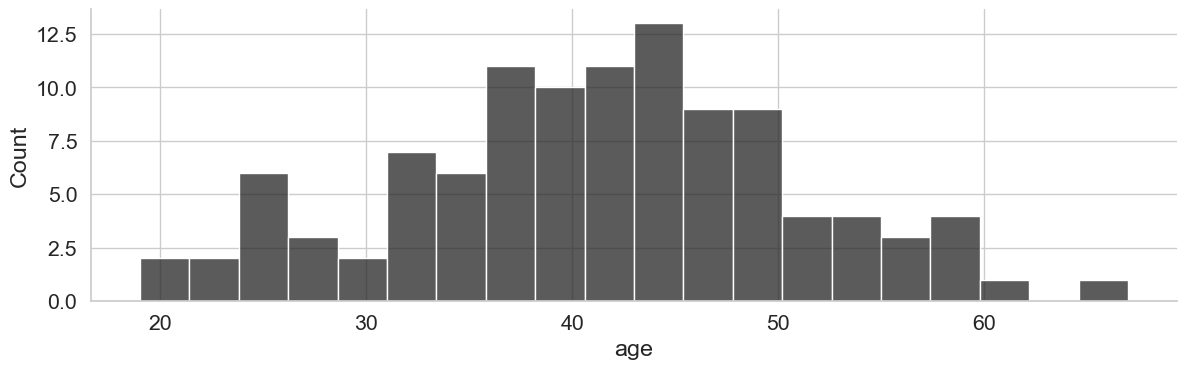
\includegraphics[height=50mm]{./figure/sec4/respondent_dist.png}
%     \caption{被験者の年齢分布}
%     \label{sec4:fig:respondent_dist}
% \end{figure}

% 次に、手法ごとの明瞭性における評価値分布を図~\ref{sec4:fig:int_score_pct}に示す。この図は横軸をモデルのID、縦軸を評価値の割合としてプロットしたものである。また、図~\ref{sec4:fig:int_summary_stats}に手法ごとの明瞭性における評価値平均と95\%信頼区間をプロットしたグラフ、表\ref{sec4:tab:int_summary_stats}にその具体的な値をそれぞれ示す。この図は横軸をモデルのID、縦軸を評価値としてプロットしたものである。どちらの図についても評価値平均が小さい順に左から並べてプロットしている。これより、左から合成音声が並んでおり、(4)分析合成、(5)原音声が合成音声と比較して高い評価を受けている傾向が見て取れる。自然性についても同様に、評価値分布を図~\ref{sec4:fig:nat_score_pct}、評価値平均と95\%信頼区間を図~\ref{sec4:fig:nat_summary_stats}、表\ref{sec4:tab:nat_summary_stats}にそれぞれ示す。自然性についても明瞭性と同様の傾向が見て取れる。原音声の評価値が最も高く、ついで分析合成、合成音声となることは実験として妥当な結果であり、実験は問題なく行われたと判断した。

% \begin{figure}[bt]
%     \centering
%     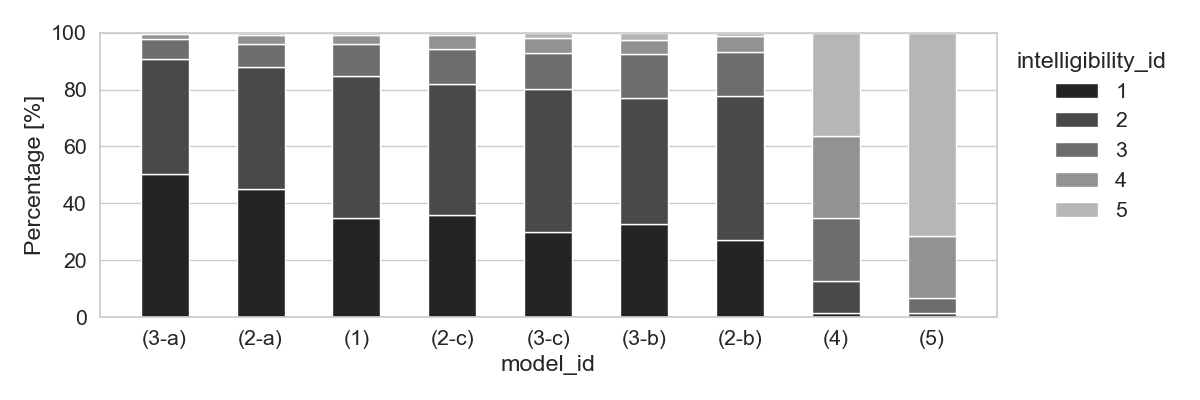
\includegraphics[height=50mm]{./figure/sec4/int_score_pct.png}
%     \caption{手法ごとの明瞭性における評価値分布}
%     \label{sec4:fig:int_score_pct}
% \end{figure}

% \begin{figure}[bt]
%     \centering
%     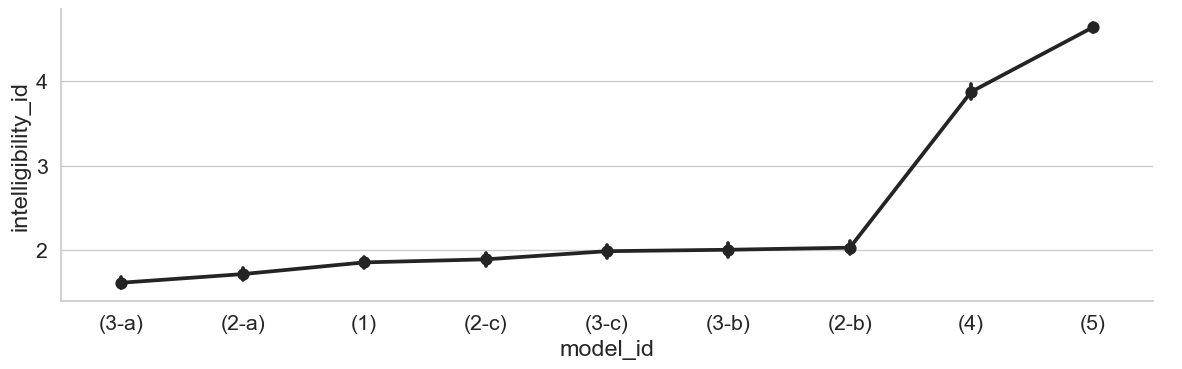
\includegraphics[height=50mm]{./figure/sec4/int_summary_stats.png}
%     \caption{手法ごとの明瞭性における評価値平均と95\%信頼区間(グラフ)}
%     \label{sec4:fig:int_summary_stats}
% \end{figure}

% \begin{table*}[bt]
%     \centering
%     \caption{手法ごとの明瞭性における評価値平均と95\%信頼区間}
%     \label{sec4:tab:int_summary_stats}
%     \begin{center}
%         \renewcommand{\arraystretch}{1.0} % 行の高さ調整
%         \setlength{\tabcolsep}{8pt}      % 列の幅調整
%         \scalebox{0.9}{
%             \begin{tabular}{|l|l|l|r|}
%                 \hline
%                 \multicolumn{1}{|c|}{ID} & \multicolumn{1}{c|}{手法} & \multicolumn{1}{c|}{予測対象} & \multicolumn{1}{c|}{評価値} \\
%                 \hline
%                 (3-a)                    & HuBERTあり                & メル・連続                     & $1.61 \pm 0.03$          \\
%                 (2-a)                    & HuBERTなし                & メル・連続                     & $1.72 \pm 0.04$          \\
%                 (1)                      & ベースライン                  & メル                        & $1.85 \pm 0.04$          \\
%                 (2-c)                    & HuBERTなし                & メル・連続・離散                  & $1.89 \pm 0.04$          \\
%                 (3-c)                    & HuBERTあり                & メル・連続・離散                  & $1.99 \pm 0.04$          \\
%                 (3-b)                    & HuBERTあり                & メル・離散                     & $2.00 \pm 0.04$          \\
%                 (2-b)                    & HuBERTなし                & メル・離散                     & $2.03 \pm 0.04$          \\
%                 (4)                      & 分析合成                    & \multicolumn{1}{c|}{-}    & $3.87 \pm 0.05$          \\
%                 (5)                      & 原音声                     & \multicolumn{1}{c|}{-}    & $4.63 \pm 0.03$          \\
%                 \hline
%             \end{tabular}
%         }
%     \end{center}
% \end{table*}

% \begin{figure}[bt]
%     \centering
%     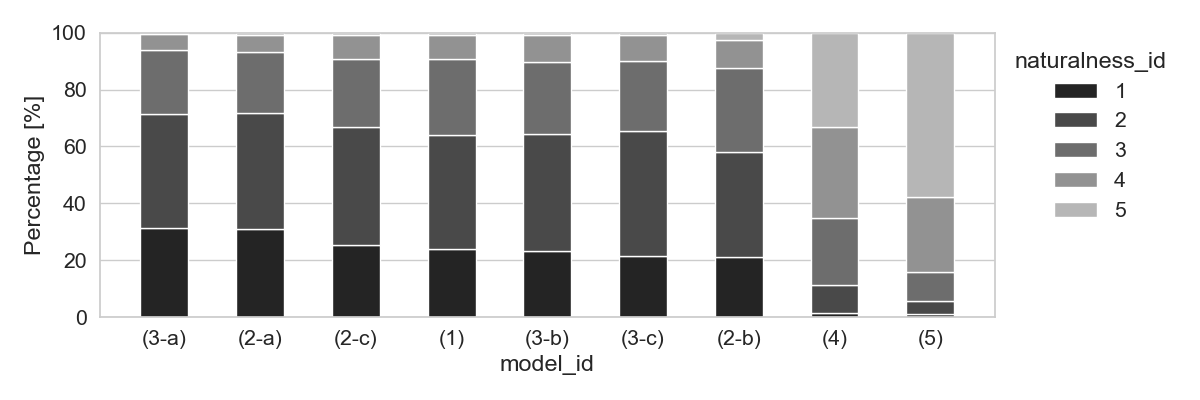
\includegraphics[height=50mm]{./figure/sec4/nat_score_pct.png}
%     \caption{手法ごとの自然性における評価値分布}
%     \label{sec4:fig:nat_score_pct}
% \end{figure}

% \begin{figure}[bt]
%     \centering
%     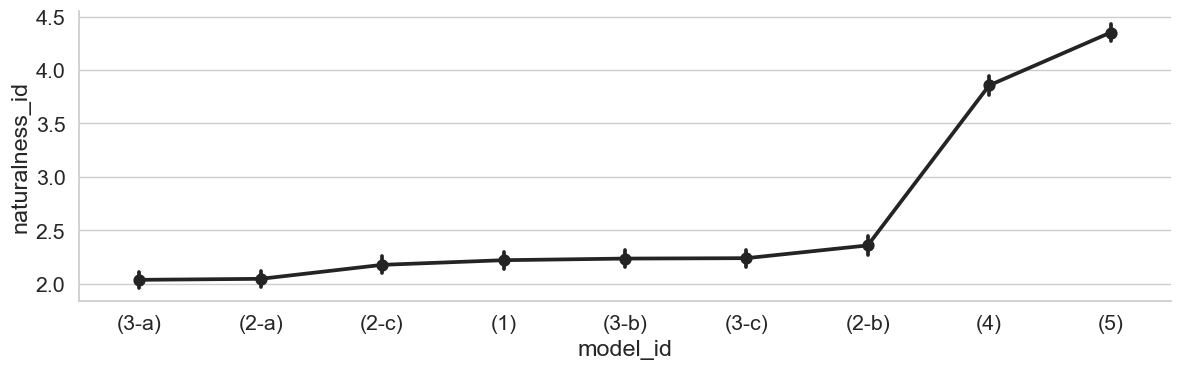
\includegraphics[height=50mm]{./figure/sec4/nat_summary_stats.png}
%     \caption{手法ごとの自然性における評価値平均と95\%信頼区間(グラフ)}
%     \label{sec4:fig:nat_summary_stats}
% \end{figure}

% \begin{table*}[bt]
%     \centering
%     \caption{手法ごとの自然性における評価値平均と95\%信頼区間}
%     \label{sec4:tab:nat_summary_stats}
%     \begin{center}
%         \renewcommand{\arraystretch}{1.0} % 行の高さ調整
%         \setlength{\tabcolsep}{8pt}      % 列の幅調整
%         \scalebox{0.9}{
%             \begin{tabular}{|l|l|l|r|}
%                 \hline
%                 \multicolumn{1}{|c|}{ID} & \multicolumn{1}{c|}{手法} & \multicolumn{1}{c|}{予測対象} & \multicolumn{1}{c|}{評価値} \\
%                 \hline
%                 (3-a)                    & HuBERTあり                & メル・連続                     & $2.04 \pm 0.04$          \\
%                 (2-a)                    & HuBERTなし                & メル・連続                     & $2.05 \pm 0.04$          \\
%                 (2-c)                    & HuBERTなし                & メル・連続・離散                  & $2.18 \pm 0.04$          \\
%                 (1)                      & ベースライン                  & メル                        & $2.22 \pm 0.04$          \\
%                 (3-b)                    & HuBERTあり                & メル・離散                     & $2.24 \pm 0.04$          \\
%                 (3-c)                    & HuBERTあり                & メル・連続・離散                  & $2.24 \pm 0.04$          \\
%                 (2-b)                    & HuBERTなし                & メル・離散                     & $2.36 \pm 0.04$          \\
%                 (4)                      & 分析合成                    & \multicolumn{1}{c|}{-}    & $3.86 \pm 0.05$          \\
%                 (5)                      & 原音声                     & \multicolumn{1}{c|}{-}    & $4.35 \pm 0.04$          \\
%                 \hline
%             \end{tabular}
%         }
%     \end{center}
% \end{table*}

% この評価データを用いて評価値平均に対するt検定を実施することで、手法間の有意差の有無を評価した。手法間で回答者は同じではないため、二群間が等分散であることを仮定しないウェルチのt検定を実施した。また、平均値が大きい手法について、それが統計的に有意な差であるかに興味があるため、有意水準5\%で片側検定を実施した。加えて、手法の組み合わせが多数存在することから、Benjamini-Hochberg法によってp値を補正した。得られたp値をまとめた結果が、表~\ref{sec4:tab:int_ttest}, ~\ref{sec4:tab:nat_ttest}である。この表のi行j列に示す値は、手法i、jの評価平均をそれぞれ$\mu_{i}$、$\mu_{j}$とすると、帰無仮説を「$\mu_{i} = \mu_{j}$」、対立仮説を「$\mu_{i} > \mu_{j}$」とした時のp値である。有意水準5\%で有意差が認められた組み合わせは、下線を引いて示している。

% この結果に対して、以下の三つの観点で考える。
% \begin{enumerate}
%     \item 最も評価の高かった手法は何だったか
%     \item HuBERT導入による効果はあったか
%     \item 予測対象の違いは合成音声の品質に影響を与えたか
% \end{enumerate}

% まず、最も評価の高かった手法は何だったかについて、表~\ref{sec4:tab:int_ttest}を見ると、手法(2-b)、(3-b)、(3-c)がその他の4つの手法に対して有意に評価が高いことが分かる。これより、これら三つの手法はその他の4つの合成音声と比較して、明瞭性が高かったと考えられる。さらに、表~\ref{sec4:tab:nat_ttest}を見ると、手法(2-b)がその他の6つの手法に対して有意に評価が高いことが分かる。これより、評価対象とした合成音声の中で、(2-b)は最も自然性が高かったと考えられる。以上の結果から、今回比較した手法の中で最も評価が高かったのは(2-b)だと考えられ、これはHuBERTなしで音声SSL離散特徴量を予測対象とした先行研究~\cite{choi2023intelligible}の手法である。これは先行研究~\cite{choi2023intelligible}の有効性の指示する結果となり、本研究で新たに提案したHuBERTを導入するアプローチは、この手法を超えることができなかったと言える。

% 次に、HuBERT導入による効果について調べるため、同じ予測対象でHuBERTの有無のみに違いがある、(2-a)と(3-a)、(2-b)と(3-b)、(2-c)と(3-c)の間における有意差の有無に着目する。これら3つのペアのみにおける有意差の有無をまとめた結果を表~\ref{sec4:tab:ttest_hubert}に示す。ここでは有意差のある場合を不等号、ない場合を等号で示している。まず、(2-a)と(3-a)の結果を見ると、明瞭性では(2-a)が有意に高く、自然性では有意差がないことが分かる。次に、(2-b)と(3-b)の結果を見ると、明瞭性では有意差がなく、自然性では(2-b)が有意に高いことが分かる。これらより、HuBERTの導入によって明瞭性あるいは自然性が悪化していると考えられる。しかし、(2-c)と(3-c)の結果を見ると、明瞭性では(3-c)が有意に高く、自然性では有意差がないことが分かる。これは前述した傾向と異なり、HuBERT導入が明瞭性の向上に寄与したと考えられる。従って、本研究で提案したHuBERT導入の有効性は、モデルの予測対象によって異なると考えられる。

% 最後に、予測対象の違いによる変化について調べるため、HuBERTの有無で共通していて予測対象のみに違いがある、(2-a)と(2-b)と(2-c)、(3-a)と(3-b)と(3-c)の間における有意差の有無に着目した。この結果を表~\ref{sec4:tab:ttest_pred}に示す。ここでも有意差のある場合を不等号、ない場合を等号で示している。まず、(2-a)と(2-b)と(2-c)の結果を見ると、明瞭性・自然性どちらにおいても共通して、(2-b)が最も有意に高く、ついで(2-c)、(2-a)が続いて有意に低くなっていることが分かる。これより、HuBERTなしの条件下では予測対象の違いによって明瞭性・自然性ともに有意差が出ており、今回の条件下ではメルスペクトログラムと音声SSL離散特徴量を予測対象とした場合が最も良い評価を得たと言える。次に、(3-a)と(3-b)と(3-c)の結果を見ると、明瞭性・自然性ともに(3-b)と(3-c)の有意差がなくなっていることが分かる。この点がHuBERTなしの場合との違いであり、音声SSL離散特徴量のみを予測対象とする場合と、離散特徴量と連続特徴量の両方を使うアプローチにおける差が小さくなったと考えられる。最後に、メルスペクトログラムと音声SSL連続特徴量を予測対象とした(2-a)、(3-a)はHuBERTの有無によらず有意に評価が低くなっていることが分かる。これより、音声SSLモデルから得られる特徴量を連続値のまま予測対象とするアプローチは、離散化させるアプローチと比較して有効でないと考えられる。連続特徴量はそれを離散化させた特徴量と比較して、より複雑であることが予想される。これを正確に推定しようとするよりも、離散化させてある程度冗長性を省いたものを予測対象とした方が、結果的に合成音声の品質改善につながるのだと考えられる。

% \begin{table*}[bt]
%     \centering
%     \caption{明瞭性の評価値平均に対するt検定の結果}
%     \label{sec4:tab:int_ttest}
%     \begin{center}
%         \renewcommand{\arraystretch}{1.0} % 行の高さ調整
%         \setlength{\tabcolsep}{8pt}      % 列の幅調整
%         \scalebox{0.65}{
%             \begin{tabular}{|l|l|l|l|l|l|l|l|l|l|}
%                 \hline
%                       & \multicolumn{1}{c|}{(4)}    & \multicolumn{1}{c|}{(2-b)}  & \multicolumn{1}{c|}{(3-b)}  & \multicolumn{1}{c|}{(3-c)}  & \multicolumn{1}{c|}{(2-c)}  & \multicolumn{1}{c|}{(1)}    & \multicolumn{1}{c|}{(2-a)}  & \multicolumn{1}{c|}{(3-a)}  \\
%                 \hline
%                 (5)   & \underline{\num{4.52e-40 }} & \underline{\num{9.47e-303}} & \underline{\num{4.67e-280}} & \underline{\num{2.23e-298}} & \underline{\num{1.41e-320}} & \underline{0.00           } & \underline{0.00           } & \underline{0.00           } \\
%                 (4)   & \multicolumn{1}{c|}{-}      & \underline{\num{2.12e-147}} & \underline{\num{4.99e-143}} & \underline{\num{1.22e-149}} & \underline{\num{1.50e-163}} & \underline{\num{3.73e-172}} & \underline{\num{3.92e-188}} & \underline{\num{8.84e-205}} \\
%                 (2-b) & \multicolumn{1}{c|}{-}      & \multicolumn{1}{c|}{-}      & 0.34                        & 0.24                        & \underline{\num{6.06e-03 }} & \underline{\num{5.27e-04 }} & \underline{\num{1.63e-09 }} & \underline{\num{1.32e-16 }} \\
%                 (3-b) & \multicolumn{1}{c|}{-}      & \multicolumn{1}{c|}{-}      & \multicolumn{1}{c|}{-}      & 0.38                        & \underline{0.02           } & \underline{\num{3.92e-03 }} & \underline{\num{1.14e-07 }} & \underline{\num{1.63e-13 }} \\
%                 (3-c) & \multicolumn{1}{c|}{-}      & \multicolumn{1}{c|}{-}      & \multicolumn{1}{c|}{-}      & \multicolumn{1}{c|}{-}      & \underline{0.04           } & \underline{\num{7.19e-03 }} & \underline{\num{2.32e-07 }} & \underline{\num{2.34e-13 }} \\
%                 (2-c) & \multicolumn{1}{c|}{-}      & \multicolumn{1}{c|}{-}      & \multicolumn{1}{c|}{-}      & \multicolumn{1}{c|}{-}      & \multicolumn{1}{c|}{-}      & 0.26                        & \underline{\num{5.27e-04 }} & \underline{\num{2.07e-08 }} \\
%                 (1)   & \multicolumn{1}{c|}{-}      & \multicolumn{1}{c|}{-}      & \multicolumn{1}{c|}{-}      & \multicolumn{1}{c|}{-}      & \multicolumn{1}{c|}{-}      & \multicolumn{1}{c|}{-}      & \underline{\num{3.71e-03 }} & \underline{\num{3.29e-07 }} \\
%                 (2-a) & \multicolumn{1}{c|}{-}      & \multicolumn{1}{c|}{-}      & \multicolumn{1}{c|}{-}      & \multicolumn{1}{c|}{-}      & \multicolumn{1}{c|}{-}      & \multicolumn{1}{c|}{-}      & \multicolumn{1}{c|}{-}      & \underline{0.02           } \\
%                 \hline
%             \end{tabular}
%         }
%     \end{center}
% \end{table*}

% \begin{table*}[bt]
%     \centering
%     \caption{自然性の評価値平均に対するt検定の結果}
%     \label{sec4:tab:nat_ttest}
%     \begin{center}
%         \renewcommand{\arraystretch}{1.0} % 行の高さ調整
%         \setlength{\tabcolsep}{8pt}      % 列の幅調整
%         \scalebox{0.65}{
%             \begin{tabular}{|l|l|l|l|l|l|l|l|l|l|}
%                 \hline
%                       & \multicolumn{1}{c|}{(4)}    & \multicolumn{1}{c|}{(2-b)}  & \multicolumn{1}{c|}{(3-c)}  & \multicolumn{1}{c|}{(3-b)}  & \multicolumn{1}{c|}{(1)}    & \multicolumn{1}{c|}{(2-c)}  & \multicolumn{1}{c|}{(2-a)}  & \multicolumn{1}{c|}{(3-a)}  \\
%                 \hline
%                 (5)   & \underline{\num{7.94e-16 }} & \underline{\num{1.21e-168}} & \underline{\num{1.24e-193}} & \underline{\num{2.03e-191}} & \underline{\num{5.14e-194}} & \underline{\num{2.23e-200}} & \underline{\num{3.49e-219}} & \underline{\num{1.02e-221}} \\
%                 (4)   & \multicolumn{1}{c|}{-}      & \underline{\num{6.24e-101}} & \underline{\num{3.64e-120}} & \underline{\num{4.86e-119}} & \underline{\num{3.23e-121}} & \underline{\num{8.06e-127}} & \underline{\num{1.18e-143}} & \underline{\num{1.03e-145}} \\
%                 (2-b) & \multicolumn{1}{c|}{-}      & \multicolumn{1}{c|}{-}      & \underline{0.03           } & \underline{0.03           } & \underline{0.01           } & \underline{\num{1.71e-03 }} & \underline{\num{1.41e-07 }} & \underline{\num{5.32e-08 }} \\
%                 (3-c) & \multicolumn{1}{c|}{-}      & \multicolumn{1}{c|}{-}      & \multicolumn{1}{c|}{-}      & 0.47                        & 0.40                        & 0.16                        & \underline{\num{5.79e-04 }} & \underline{\num{3.18e-04 }} \\
%                 (3-b) & \multicolumn{1}{c|}{-}      & \multicolumn{1}{c|}{-}      & \multicolumn{1}{c|}{-}      & \multicolumn{1}{c|}{-}      & 0.42                        & 0.18                        & \underline{\num{7.96e-04 }} & \underline{\num{4.47e-04 }} \\
%                 (1)   & \multicolumn{1}{c|}{-}      & \multicolumn{1}{c|}{-}      & \multicolumn{1}{c|}{-}      & \multicolumn{1}{c|}{-}      & \multicolumn{1}{c|}{-}      & 0.25                        & \underline{\num{1.71e-03 }} & \underline{\num{9.69e-04 }} \\
%                 (2-c) & \multicolumn{1}{c|}{-}      & \multicolumn{1}{c|}{-}      & \multicolumn{1}{c|}{-}      & \multicolumn{1}{c|}{-}      & \multicolumn{1}{c|}{-}      & \multicolumn{1}{c|}{-}      & \underline{0.01           } & \underline{\num{9.27e-03 }} \\
%                 (2-a) & \multicolumn{1}{c|}{-}      & \multicolumn{1}{c|}{-}      & \multicolumn{1}{c|}{-}      & \multicolumn{1}{c|}{-}      & \multicolumn{1}{c|}{-}      & \multicolumn{1}{c|}{-}      & \multicolumn{1}{c|}{-}      & 0.44                        \\
%                 \hline
%             \end{tabular}
%         }
%     \end{center}
% \end{table*}

% \begin{table*}[bt]
%     \centering
%     \caption{HuBERTの有無に対する比較}
%     \label{sec4:tab:ttest_hubert}
%     \begin{center}
%         \renewcommand{\arraystretch}{0.9} % 行の高さ調整
%         \setlength{\tabcolsep}{8pt}      % 列の幅調整
%         \scalebox{1.0}{
%             \begin{tabular}{|l|c|c|}
%                 \hline
%                             & \multicolumn{1}{c|}{明瞭性} & \multicolumn{1}{c|}{自然性} \\
%                 \hline
%                 (2-a)、(3-a) & (2-a) $>$ (3-a)          & (2-a) = (3-a)            \\
%                 (2-b)、(3-b) & (2-b) = (3-b)            & (2-b) $>$ (3-b)          \\
%                 (2-c)、(3-c) & (2-c) $<$ (3-c)          & (2-c) = (3-c)            \\
%                 \hline
%             \end{tabular}
%         }
%     \end{center}
% \end{table*}

% \begin{table*}[bt]
%     \centering
%     \caption{予測対象による比較}
%     \label{sec4:tab:ttest_pred}
%     \begin{center}
%         \renewcommand{\arraystretch}{0.9} % 行の高さ調整
%         \setlength{\tabcolsep}{8pt}      % 列の幅調整
%         \scalebox{1.0}{
%             \begin{tabular}{|l|c|c|}
%                 \hline
%                                   & \multicolumn{1}{c|}{明瞭性}  & \multicolumn{1}{c|}{自然性}  \\
%                 \hline
%                 (2-a)、(2-b)、(2-c) & (2-b) $>$ (2-c) $>$ (2-a) & (2-b) $>$ (2-c) $>$ (2-a) \\
%                 (3-a)、(3-b)、(3-c) & (3-b) = (3-c) $>$ (3-a)   & (3-b) = (3-c) $>$ (3-a)   \\
%                 \hline
%             \end{tabular}
%         }
%     \end{center}
% \end{table*}

% \clearpage

% \subsection{まとめ}
% 本章では、音声SSLモデルであるHuBERTを利用した動画音声合成モデルを提案し、既存手法との比較を行った。

% 客観評価では、HuBERTを利用してメルスペクトログラムと音声SSL連続特徴量、離散特徴量を予測対象とした手法が、PESQ、STOI、ESTOIにおいて最も高い評価を得た。しかし、WERにおいてはHuBERTなしでメルスペクトログラムと音声SSL離散特徴量を予測対象とした手法が最も低く、提案手法に課題が残った。主観評価では、客観評価においてWERが最も低かった、HuBERTなしでメルスペクトログラムと音声SSL離散特徴量を予測対象とした手法が最も高い評価を得た。本研究で提案した手法もそれに次ぐような評価ではあったが、特に自然性については有意に低く、既存手法に対する提案手法の有効性は示されなかった。また、HuBERTの導入による効果の良し悪しはモデルの予測対象によって異なること、予測対象として音声SSL連続特徴量を直接推定するアプローチでは有効ではなさそうだということがわかった。

% 今後の研究では、提案手法の更なる改善に取り組む必要があると考える。本章では、改めて既存手法の有効性が示されたものの、得られる合成音声の品質は未だ低い。実際、主観評価実験の結果から、分析合成や原音声と合成音声の間の差は顕著であることが分かる。代用音声として利用する上ではより自然な音声であることが望ましく、既存手法を超える品質を達成する、新たな手法の検討が今後も必要だと考える。また、提案手法について課題が残る結果となったが、学習方法や予測方法に改善の余地があるのではないかと考えている。例えば、今回のHuBERTの学習ではすべての重みを更新するようFineTuningしたが、少量の音声データでチューニングした結果として、事前学習によって得た知識を忘却してしまう破滅的忘却に陥っていた可能性があり、これを防止するような学習を施すことが有効な可能性がある。また、HuBERTの事前学習ではマスク部分を推定するが、この際には正しいフレームを参照可能である。しかし、今回のFineTuningでは初めから推定結果のみを入力としていたため正しいフレームが存在せず、この条件のギャップが転移学習を困難にしていた可能性がある。これに対して、初めは合成音声にあえて原音声を混入させたものを入力として学習し、それを徐々に完全な合成音声に近づけるような方法ならば、転移学習をより効果的に行える可能性がある。最後に、今回はHuBERTのみから音声SSL特徴量を推定するような形でネットワークを提案したが、AVHuBERTから同時に予測するような枠組みとしても良いと考えている。先行研究が有効であったことも考慮すると、AVHuBERTから予測した結果とHuBERTから予測した結果を両方利用するようなアプローチも、改善の可能性があると考える。

% \clearpage

% \section{音声SSLモデルを活用した動画音声合成の再検討}
% \subsection{客観評価指標の見直し}
% これまでに用いてきた四つの客観評価指標は、動画音声合成において一般的に用いられていることから採用していた。しかし、音声合成において本質的に重要なのは、人が実際に聞いた上で良いと思うか、すなわち主観評価の良し悪しであると考える。そこで、主観評価実験における評価平均値と、客観評価指標の間で計算した相関係数を表に示す。
% これより、明瞭性においてはESTOIおよびWERの相関係数の絶対値が0.9と同程度に高く、PESQやSTOIはこれらと比較して相関係数の絶対値が小さい。
% また、自然性においてはWERの相関係数の絶対値が0.911と再び高いが、PESQ、STOI、ESTOIはこれと比較して相関係数の絶対値が小さい。
% 以上の結果から、従来一般的に用いられてきた客観評価指標の中でPESQ、STOI、ESTOIは主観評価との相関が比較的弱く、主観評価実験に向けたモデルのチューニングを行っていく上では、WERが最も信頼できる指標であると判断する。
% 加えて、表では近年提案されたMOS値の自動評価モデルである、UTMOSによって得られた評価値についての相関係数も掲載している。これを見ると、特に明瞭性においてその相関係数は0.986と高く、自然性との相関係数も0.882となっており、WERと同程度の高い値を示している。
% これより、本セクション以降ではこれまで用いてきた客観評価指標を改め、主観評価との相関が高いWERとUTMOSによって合成音声の客観評価を行うこととする。

% \begin{table*}[b]
%     \centering
%     \caption{予測対象による比較}
%     \label{sec5:tab:obj_comp}
%     \begin{center}
%         \renewcommand{\arraystretch}{0.9} % 行の高さ調整
%         \setlength{\tabcolsep}{8pt}      % 列の幅調整
%         \scalebox{1.0}{
%             \begin{tabular}{|l|c|c|}
%                 \hline
%                       & \multicolumn{1}{c|}{明瞭性} & \multicolumn{1}{c|}{自然性} \\
%                 \hline
%                 PESQ  & 0.671                    & 0.523                    \\
%                 STOI  & 0.690                    & 0.676                    \\
%                 ESTOI & 0.900                    & 0.749                    \\
%                 WER   & -0.900                   & -0.911                   \\
%                 UTMOS & 0.986                    & 0.882                    \\
%                 \hline
%             \end{tabular}
%         }
%     \end{center}
% \end{table*}

% \clearpage

\section{結論}

\clearpage

\section*{謝辞}
\addcontentsline{toc}{section}{謝辞}

\clearpage

\bibliographystyle{junsrt}
\addcontentsline{toc}{section}{参考文献}
\bibliography{library}

\end{document}